\chapter{Methods}
\section{Part 1: Determination of electrode distance d from measurement of capacitance}
\label{part1}
\subsection{General approach}
The setup is illustrated in figure \ref{sec.setup_amp_1}. A metallic cell (grounded) surrounds the  epoxy resin sample and makes sure that the current flowing from the electrode to the wall flows into ground and is not measured. The DLPCA transimpedance amplifier\footnotemark converts the measured current into a voltage and amplifies it. After a butterworth filter (order 8) an ADC creates a digital output that is processed with MATLAB. The butterworth filter ensures that frequencies above 100 kHz, which are not interesting for the mixed-frequency investigation, are cut out. The butterworth filter also prevents aliasing. 
\footnotetext{Data sheet for the used DLPCA: \url{http://www.femto.de/en/products/current-amplifiers/variable-gain-up-to-500-khz-dlpca.html}}
\begin{figure}[htbp]
	\centering
	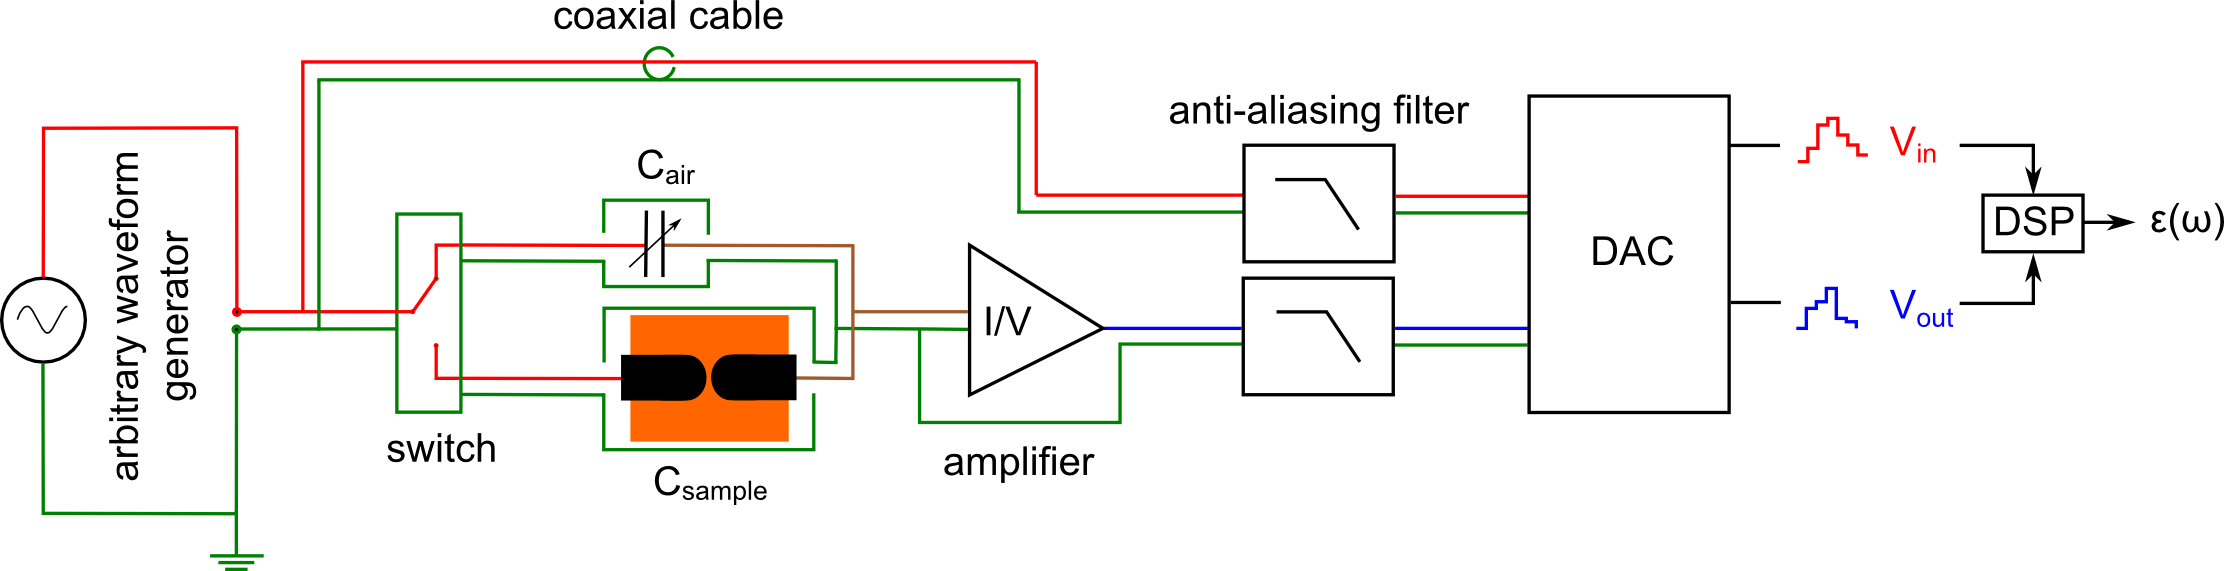
\includegraphics[width=\textwidth]{figures/Method/setup/setup_amplifier.png}		
	\caption[Kurze Abbildungsbeschreibung]{Setup for measurements with sample and DLPCA transimpedance amplifier. In this work, the setup is used to determine the capacitance of the specimen and to provide a reference for the dielectric spectroscopy measurements.\protect\footnotemark} 
	\label{sec.setup_amp_1}
\end{figure}

\label{sec:general_approach}
The following method is based on the assumption that  $\varepsilon$ is always the same for the used samples after manufacturing. Thus, it is required to determine the distance of the electrodes for each delivered sample in order to be able to calculate the effective $\varepsilon$, because the distance might vary considerably for different samples. 
At first, the initial $\varepsilon_{\textrm{eff}}$ for two reference samples has to be obtained:\\
For the two reference samples the distance is measured optically with a microscope. By using the $d-C_0$-look-up table described in  chapter \ref{sec.sim_vac_comsol} the vacuum capacitance can be obtained from the optical distance measurement. Together with the measured capacitance $C^*$ an estimation of the effective epsilon for the used epoxy resin is possible. 

For forther samples, the capacitance $C^*$ has to be measured. Together with the initial value of $\varepsilon_{\textrm{eff}}$ of the reference samples one can obtain the vacuum capacitance $C_0$. By using the $d-C_0$ look up table an estimation of the electrode distance d is possible. Now, the vacuum capacitance and the corresponding electrode distance are known for further measurements. As a consequence, it is possible to get the the values and changes in the effective permittivity with the calculated $C_0$.

\footnotetext{source: Raphael F\"arber}

\subsection{Measuring the capacitance of the sample}

$C^*$ was measured by determining the impedance of the sample with the setup described in \ref{spectroscopy} but its measurement
parameters are mentioned here for the sake of completeness of \ref{part1}.
A series of 25 measurements was conducted whereas the capacitance was removed
and re-inserted into its holder after each measurement. Each time the epoxy resin sample was
re-inserted 25 individual measurements were automatically carried out amounting to a total of 625 recordings.

\begin{figure}[h!tb]
	\centering
	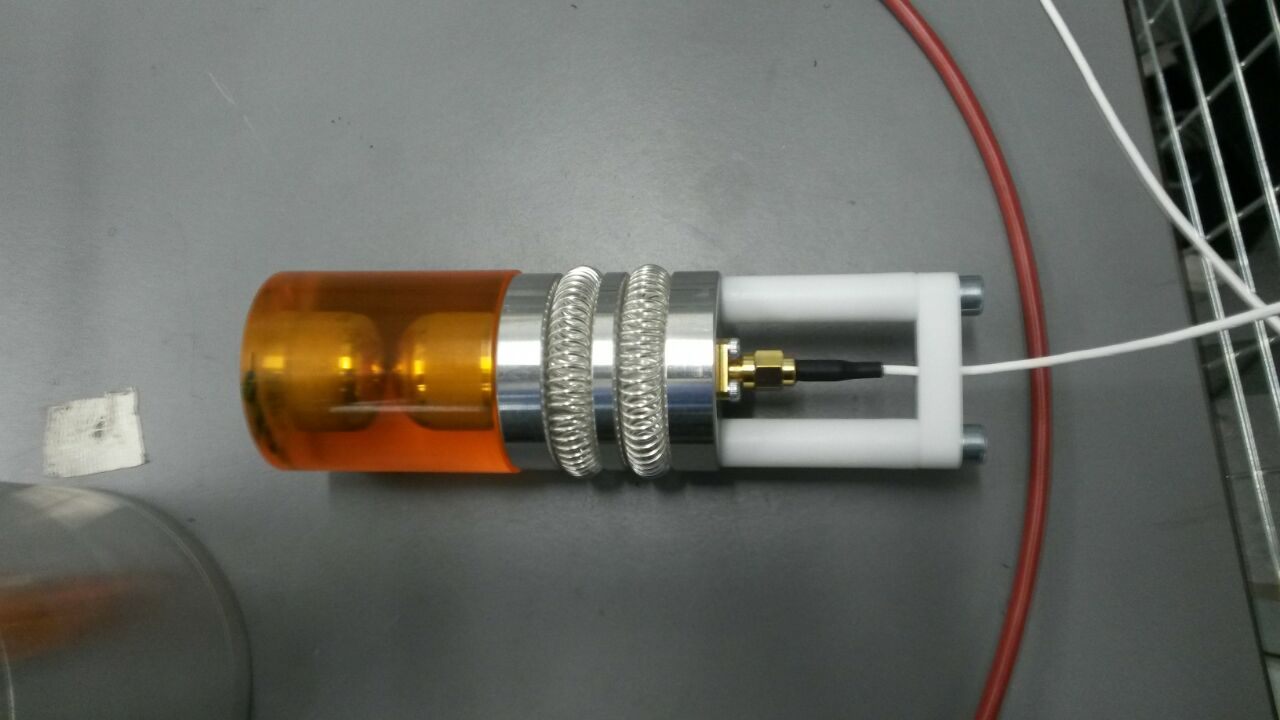
\includegraphics[width=0.8\textwidth]{figures/Method/Experimentaufbau/epoxy.jpg}		
	\caption[Kurze Abbildungsbeschreibung]{Sample of dielectric specimen on the holder} \label{fig.comsol_beispiel}

\end{figure}


\subsection{Simulation of vacuum capacitance} 
\label{sec.sim_vac_comsol}
As mentioned in the chapters before the vacuum capacitance cannot the calculated directly because of the complexity of the geometry. COMSOL is a simulation software that solves the Maxwell equations numerically and thus, is suitable for a numerical estimation of permittivities or capacitances between arbitrarily shaped electrodes. The dependency of the vacuum capacity $C_0$ on the electrode distance d has to be simulated numerically both for the high-voltage setup and for the low-voltage setup. Although all measurements and the corresponding calculations in section \ref{sec:general_approach} can be carried out in the low-voltage setup it is useful to be able to do these calculations in the high-voltage setup as well. 


\begin{figure}[htbp]
	\centering
	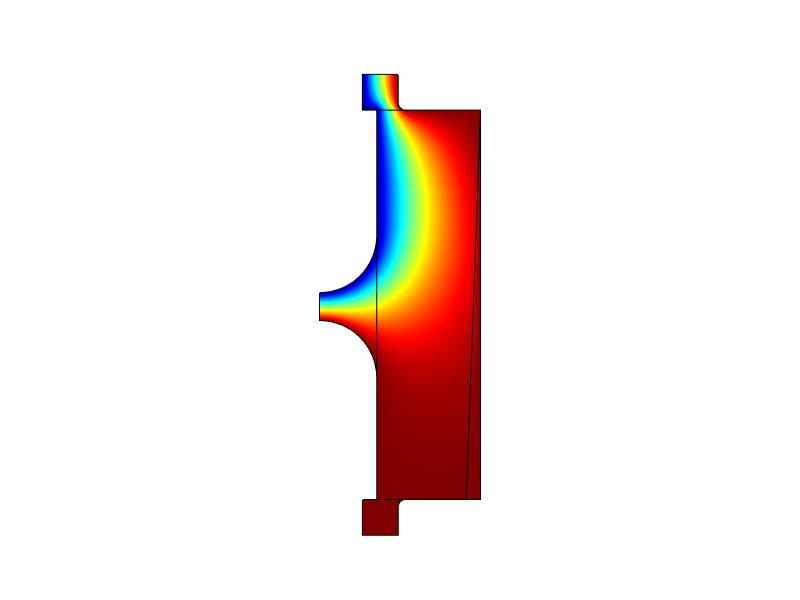
\includegraphics{figures/COMSOL_Beispielbild.jpg}		
	\caption[Kurze Abbildungsbeschreibung]{Electrical potential simulation of the low-voltage test cell with cylindrically shaped electrodes (normally 0.5 mm electrode distance)} \label{fig.comsol_beispiel}

\end{figure}
 
Figure \ref{fig.comsol_beispiel} shows the simulated electrical potential distribution in the low-voltage setup in COMSOL for an electrode with a cyclindrical geometry. Since the capacitance of the setup and therefore also the currents depend on the geometry of the electrode a conic electrode is simulated as well as shown in figure  \ref{fig.comsol_conic}

\begin{figure}[htbp]
	\centering
	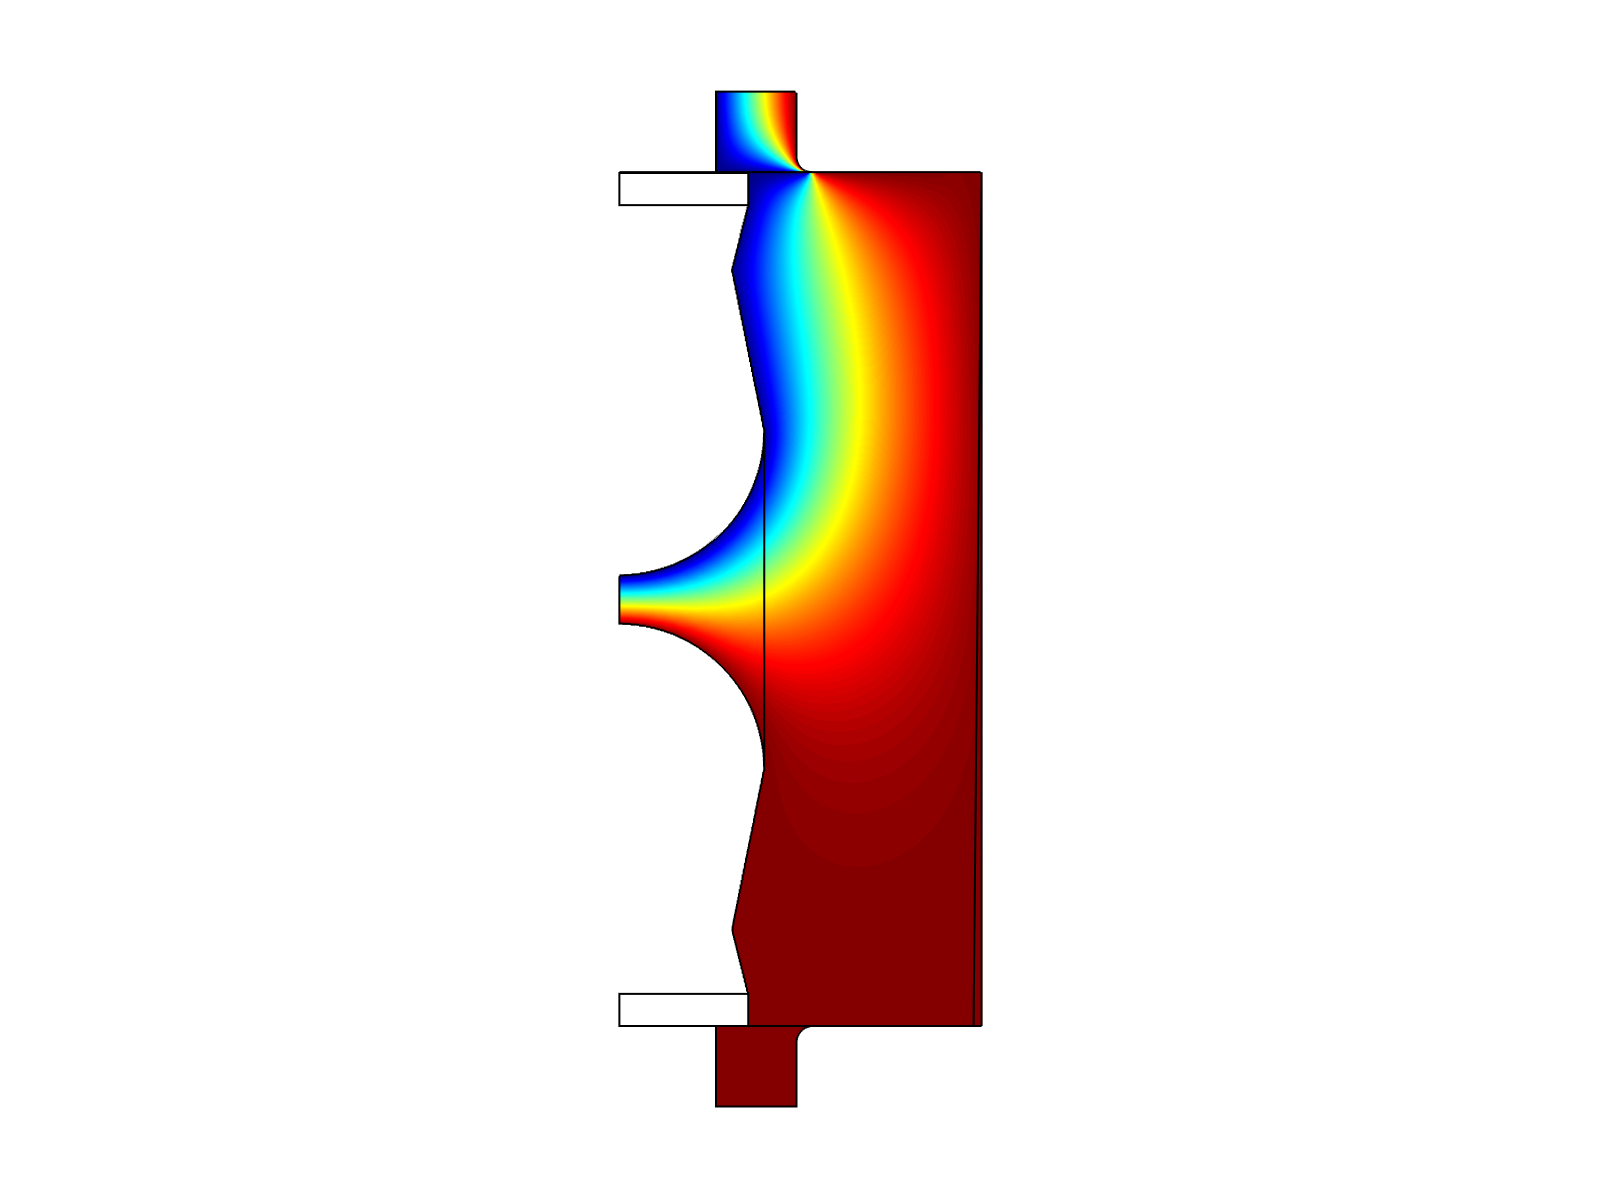
\includegraphics[scale=0.3]{figures/Method/Part1_d_C0/conic.png}		
	\caption[Kurze Abbildungsbeschreibung]{Electrical potential simulation of the low-voltage test cell with conically shaped electrodes (0.5 mm electrode distance) at } \label{fig.comsol_conic}

\end{figure}

In order to validate the simulations the capacitance of two spheres with a distance d are used as a reference. The following formula gives an approximation for the capacitance of two spheres with radius r and center distance d. \cite{Rawlins}
\begin{equation}
C=2 \pi \varepsilon r ( ln 2 + \gamma -\frac{1}{2} ln(2D-2)+O(2D-2))
\end{equation}
where D is the ratio of electrode distance over sphere diameter, i.e. $ D=\frac{d}{2r}$. As the electrodes have a spherical end with 8mm radius, the radius for the two spheres is set to 8mm as well. The simulation with two spheres is illustrated in figure \ref{fig.twospheres}.  
\begin{figure}[htbp]
	\centering
	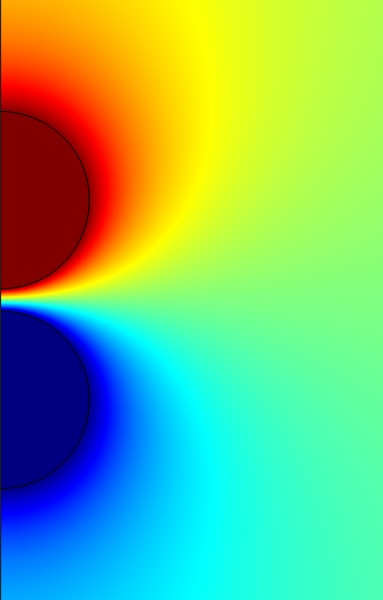
\includegraphics[scale=0.3]{figures/Method/Part1_d_C0/sphere_capacity.jpg}		
	\caption[Kurze Abbildungsbeschreibung]{Electrical potential simulation of two spheres with 8mm radius } \label{fig.comsol_sphere}
	\label{fig.twospheres}
\end{figure}


 There are several systematic errors that influence the vacuum capacitance simulation. The inclined line on the right-hand side shows the air gap that is caused during the production process. This air gap between the wall of the low-voltage setup and the specimen causes an additional inhomogeneity. It is unavoidable in order to be able to remove the specimen from the mold. This air gap is 0.5 mm. Deviations from this value (0 mm to 1 mm) were investigated with COMSOL as well. The lookup table of d based on $C_0$ is based on an air gap of 0.5 mm, therefore the deviation from this value has to be investigated numerically.
 
A stochastic error is the deviation of the height of the specimen. During  the molding process the height of the specimen cannot be fixed precisely. The maximum deviation is expected to be $\pm$ 0.5 mm. This deviation might occur during the production process of each new specimen. Thus, if the electrode distance of a specimen should be estimated by the method described these deviations can result in an error. 
 \begin{figure}[htbp]
	\centering
	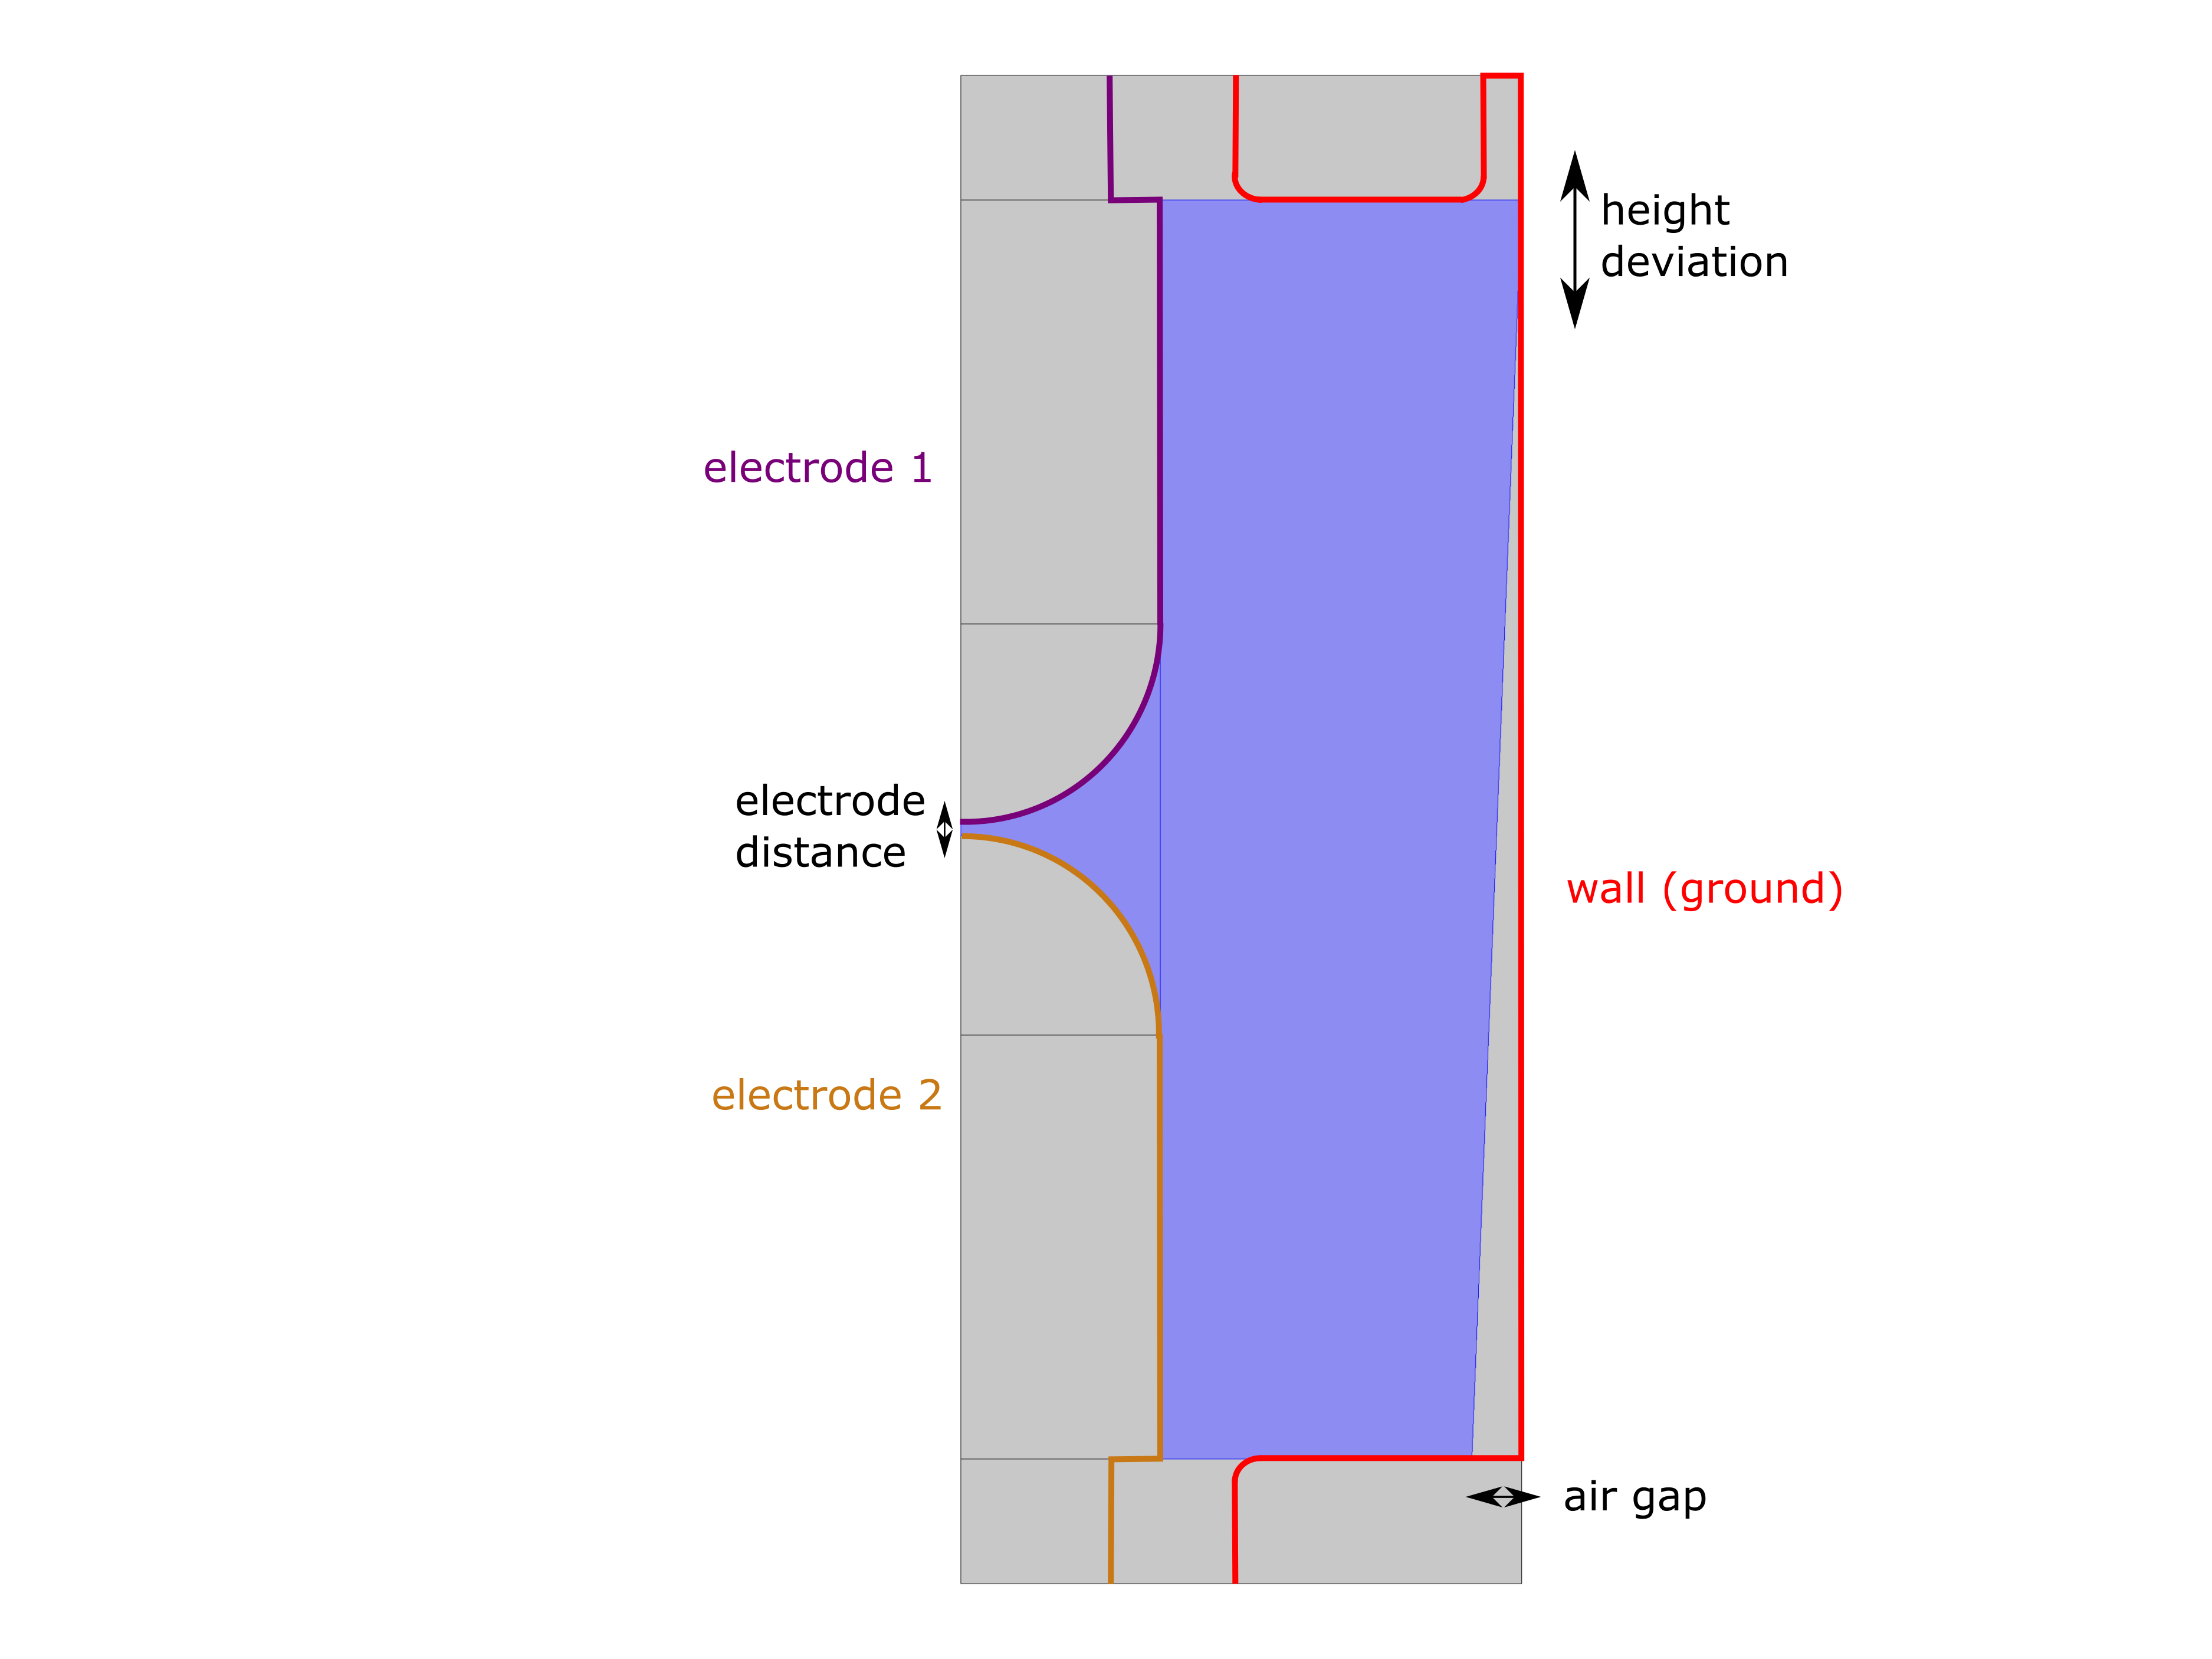
\includegraphics[width=\textwidth]{figures/Method/Part1_d_C0/cell_colour.png}		
	\caption[Kurze Abbildungsbeschreibung]{Geometry used for COMSOL simulation of the low-voltage setup} 
	\label{fig.syserrors}
\end{figure}

\section{Part 2:  Suitability of current transformers for dielectric spectroscopy}
\subsection{The setup}
There are two general setups. One is the high-voltage setup and one the low voltage-setup. For testing the suitability of the current transformer the low voltage setup is sufficient except for the clamping test described in section \ref{clamping}. There is always a reference measurement where only $C_0$ is measured (in addition to the measurement of $C_0$ plus the RC loss element). The division by a reference measurement makes sure that systematic errors in the setup, e.g. the phase shift in the current transformer, are cancelled out. 

The following figure \ref{sec.setup_amplifier} illustrates the setup for measurements without a current transformer. The DLPCA-200 is a variable gain low noise current amplifier that has a transimpedance gain between $10^3$ and $10^{11} V/A$. A MATLAB script automatically adapts its gain to a value that is suitable for the input voltage range of the ADC which is $\pm 10V$. With the values of the ADC, i.e. the input voltage of the waveform generator and the output of the BW-filter, $\varepsilon'$ and tan($\delta$) can be calculated. 

\begin{figure}[htbp]
	\centering
	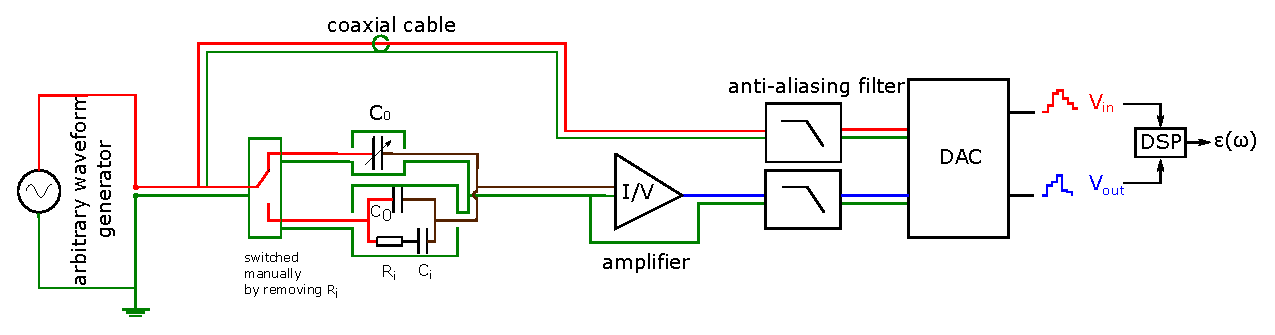
\includegraphics[width=\textwidth]{figures/Method/setup/setup_DLPCA.eps}		
	\caption[Kurze Abbildungsbeschreibung]{Setup for reference measurements \protect\footnotemark} 
	
	\label{sec.setup_amplifier}

\end{figure}

\footnotetext{source: Raphael F\"arber, revised by authors}

Afterwards, the DLPCA is replaced with a current transformer. 
\begin{figure}[htbp]
	\centering
	\includegraphics[width=\textwidth]{figures/Method/setup/setup_CTonly}		
	\caption[Kurze Abbildungsbeschreibung]{Setup for measurements with current transformer only \protect\footnotemark}
	\label{sec.setup}

\end{figure}
\footnotetext{source: Raphael F\"arber, revised by authors}

\subsection{Signal analysis of the Debye model}

In order to emulate different dielectrics with their own respective dielectric loss tangent, different combinations of circuit elements ($C_0$, $R_i$, $C_i$, $R_{\infty}$)can be used.
Each different circuit accounts for a frequency spectrum of another loss tangent with respect to frequency. With the objective to assess the performance of the current transformer, reasonably high maximal values for the $tan\left(\delta\right)$ were assumed (i.e. 0.05 to 0.2) since a lower loss tangent
would require a higher resolution on the part of the current measurement and thus, make it more difficult to assess the performance of the current transformer. The vacuum capacitance was chosen to be about 1000 times larger than
the the one of the specimen for the purpose of generating the same magnitude of currents as in the high-voltage setup.


In order to get a theoretical maximum tan($\delta$) of 0.0178 the parts shown in figure \ref{fig.debye-modell} are used. 
\begin{figure}[h!tb]
	\centerline{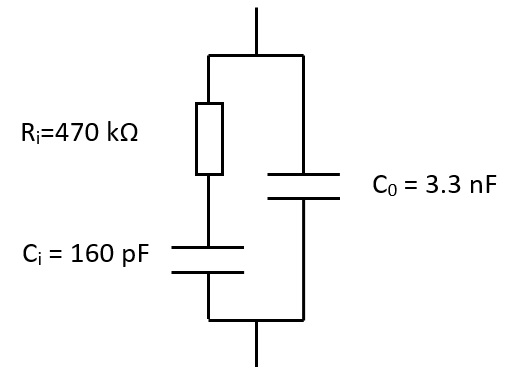
\includegraphics[width=0.5\textwidth]{figures/Method/debye-modell.jpg}}	
	\caption{Debye model for max($tan(\delta)$)=0.0178 }	
	\label{fig.debye-modellsch}
\end{figure}

Once the Debye sample  was inserted into the measurement setup of \ref{sec.setup_amplifier} we can use the schematic in \ref{fig.presentation} as a reference.

\begin{figure}[h!tb]
	\centerline{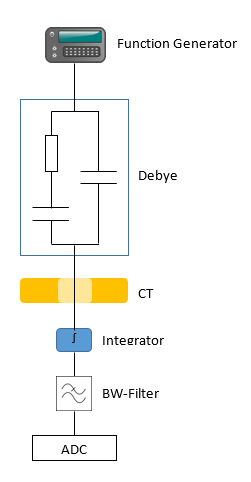
\includegraphics[width=0.4\textwidth]{figures/Method/setup/low_voltage_setup.png}}	
	\caption{Schematic setup for sectroscopy with Debye model}	
	\label{fig.presentation}
\end{figure}

While the spectroscopy was carried out primarily using sinusoidal inputs,
the practically important signals are the trapezoidal voltage pulses with different
slew rates because they occur in power electronic converters and ultimately are to be studied with this method.  Consequentially, it is relevant to predict the shape and magnitude
of the functions that are expected anywhere in the setup. 
The Debye model's parameters are assumed to be the same as in \ref{fig.debye-modellsch}.
The input trapezoidal wave's fundamental frequency is 1kHz and its amplitude was
set to 5V. Both the rise and 
the fall time are set to 1 $\mu s$. The voltage signal is created
by the function generator (model Agilent 33210) in \ref{fig.presentation}
\newline
In order to determine the current through the Debye network, the harmonic decomposition of
the trapezoidal pulse train in the theory section was used. For each harmonic, the specific
impedance of the debye network was calculated and the harmonic components for the current were found by dividing voltage component by its corresponding impedance.

\begin{equation}
 \underline{Z}_{debye}(w)=\left[\frac{1}{R_{\infty}}+\frac{1}{R_{i}+\frac{1}{jwC_{i}}}+jwC_{0}\right]^{-1}
 \label{debyeimpedance}
\end{equation}

It is important to note that $R_{\infty}$, which represents
ohmic losses in dielectrics, was intentionally set to $\infty$ in both the Debye model and calculations (no emulated DC conduction).

Figures \ref{fig.beforeandafter} and \ref{fig.fourierla} shows the voltage signal and the resulting current signal as well as their Fourier coefficients on a log-log scale.

\begin{figure}[h!tb]
\centerline{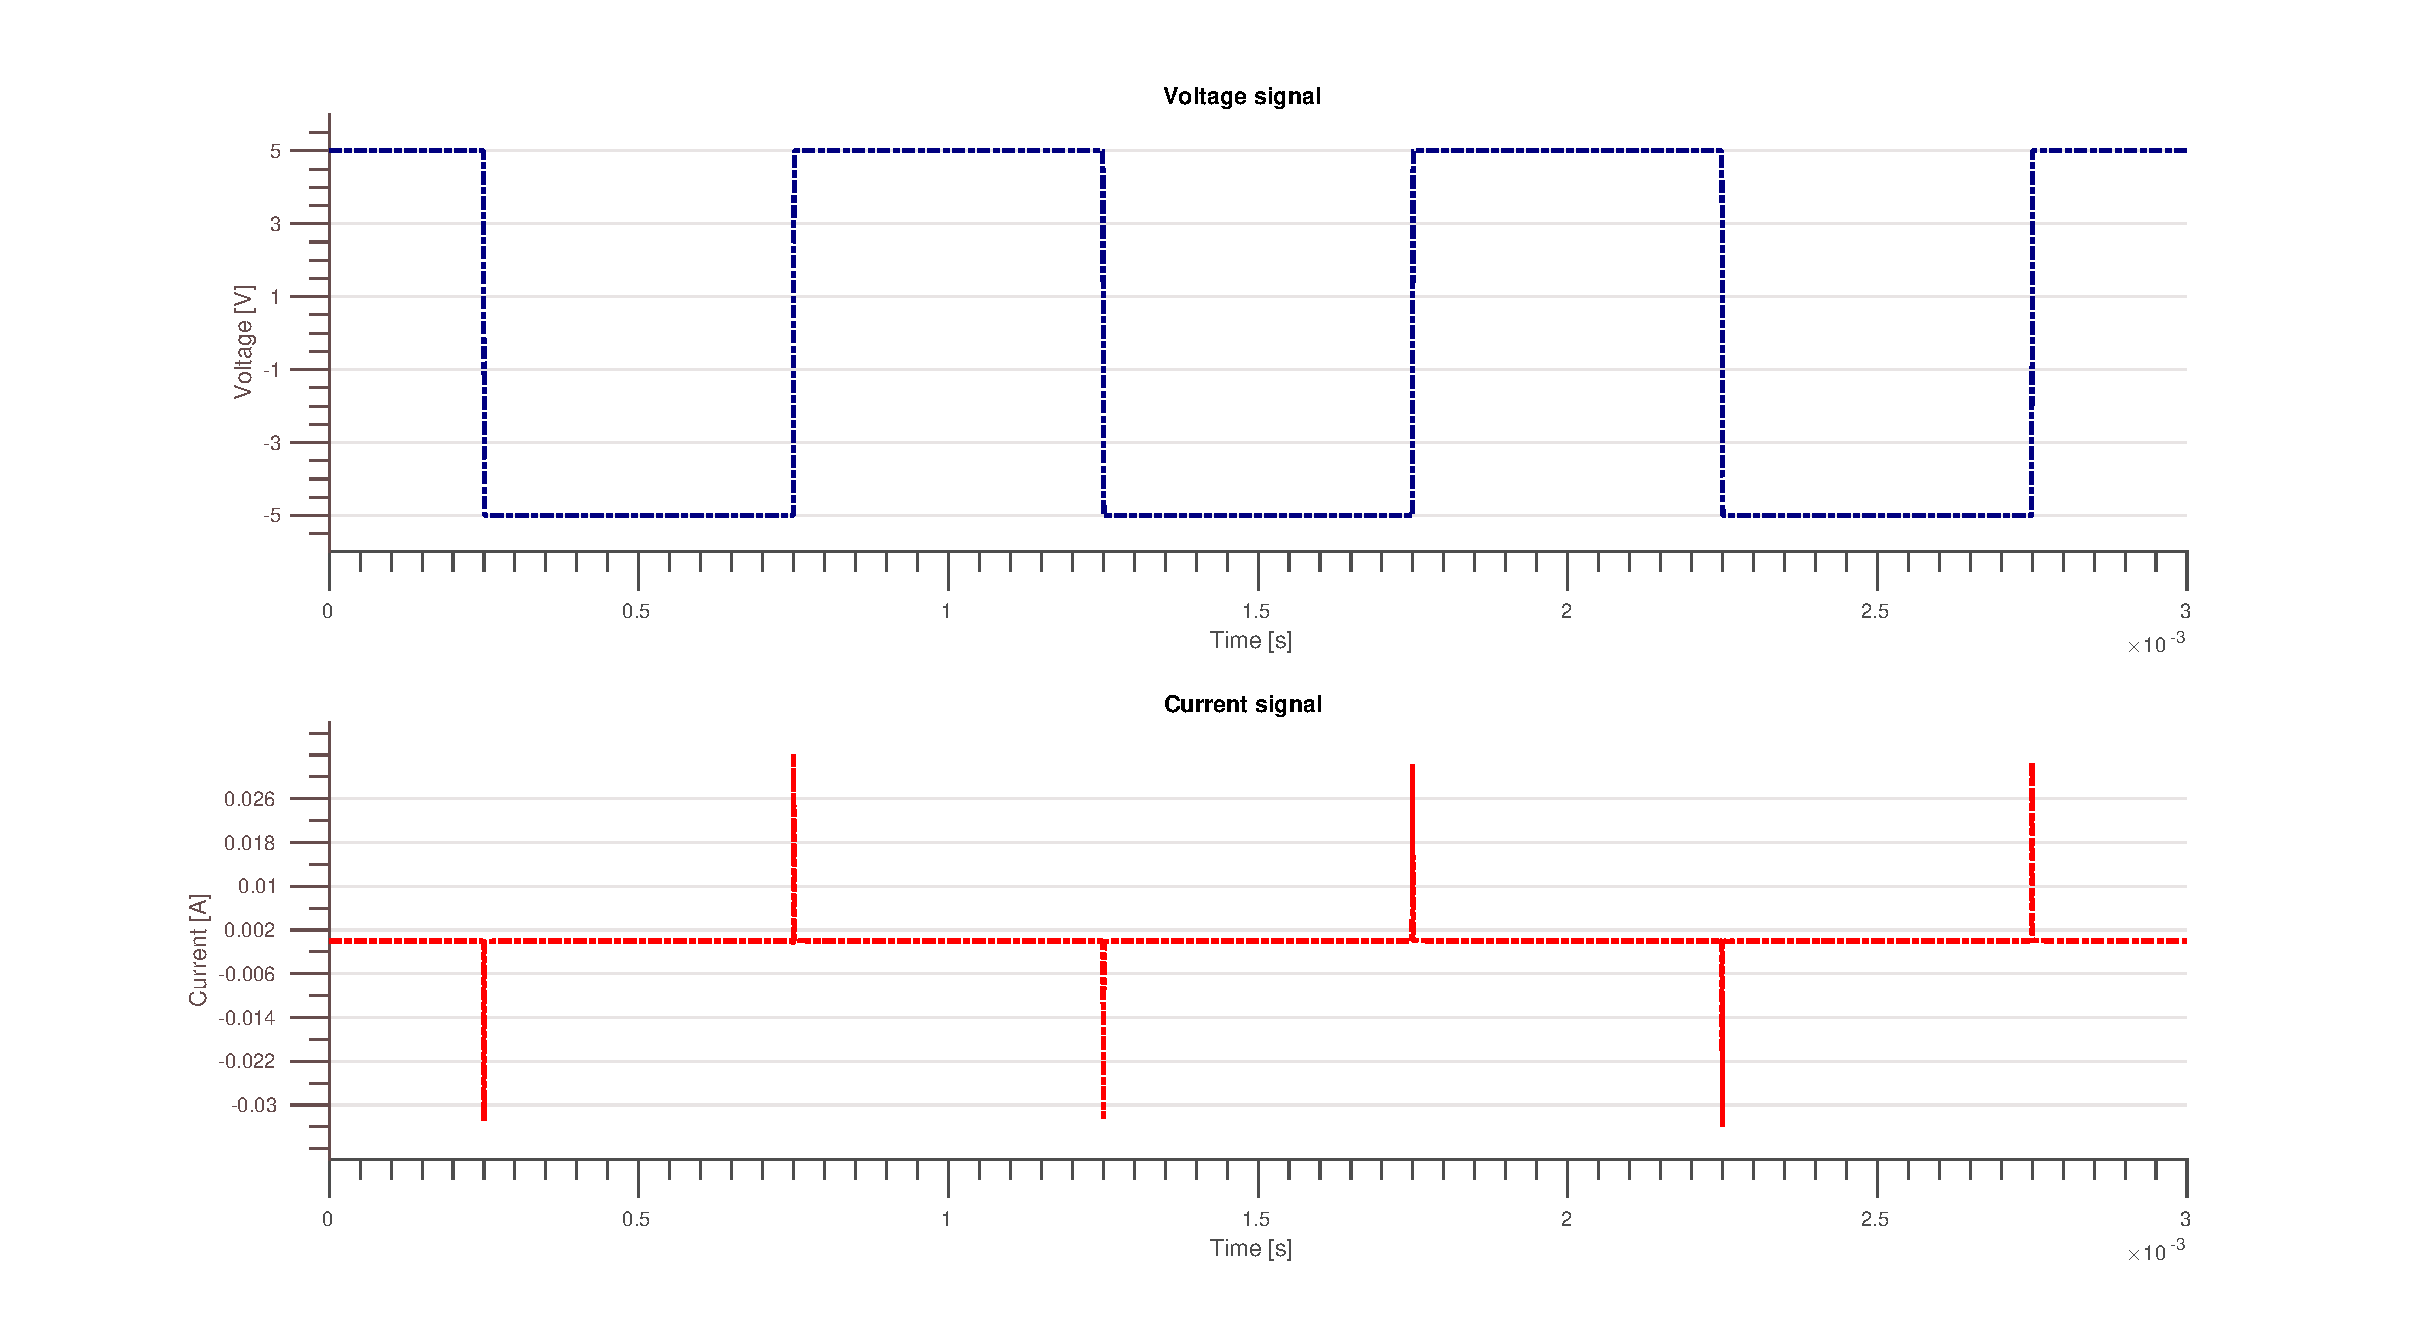
\includegraphics[width=0.8\textwidth]{figures/Method/signal_simulation/beforeandafter.eps}}
\caption{Voltage and current signals across and through debye sample. Trapzedoidal input voltage with 1 microsec. rise/fall-time}
\label{fig.beforeandafter}
\end{figure}

\begin{figure}[h!tb]
\centerline{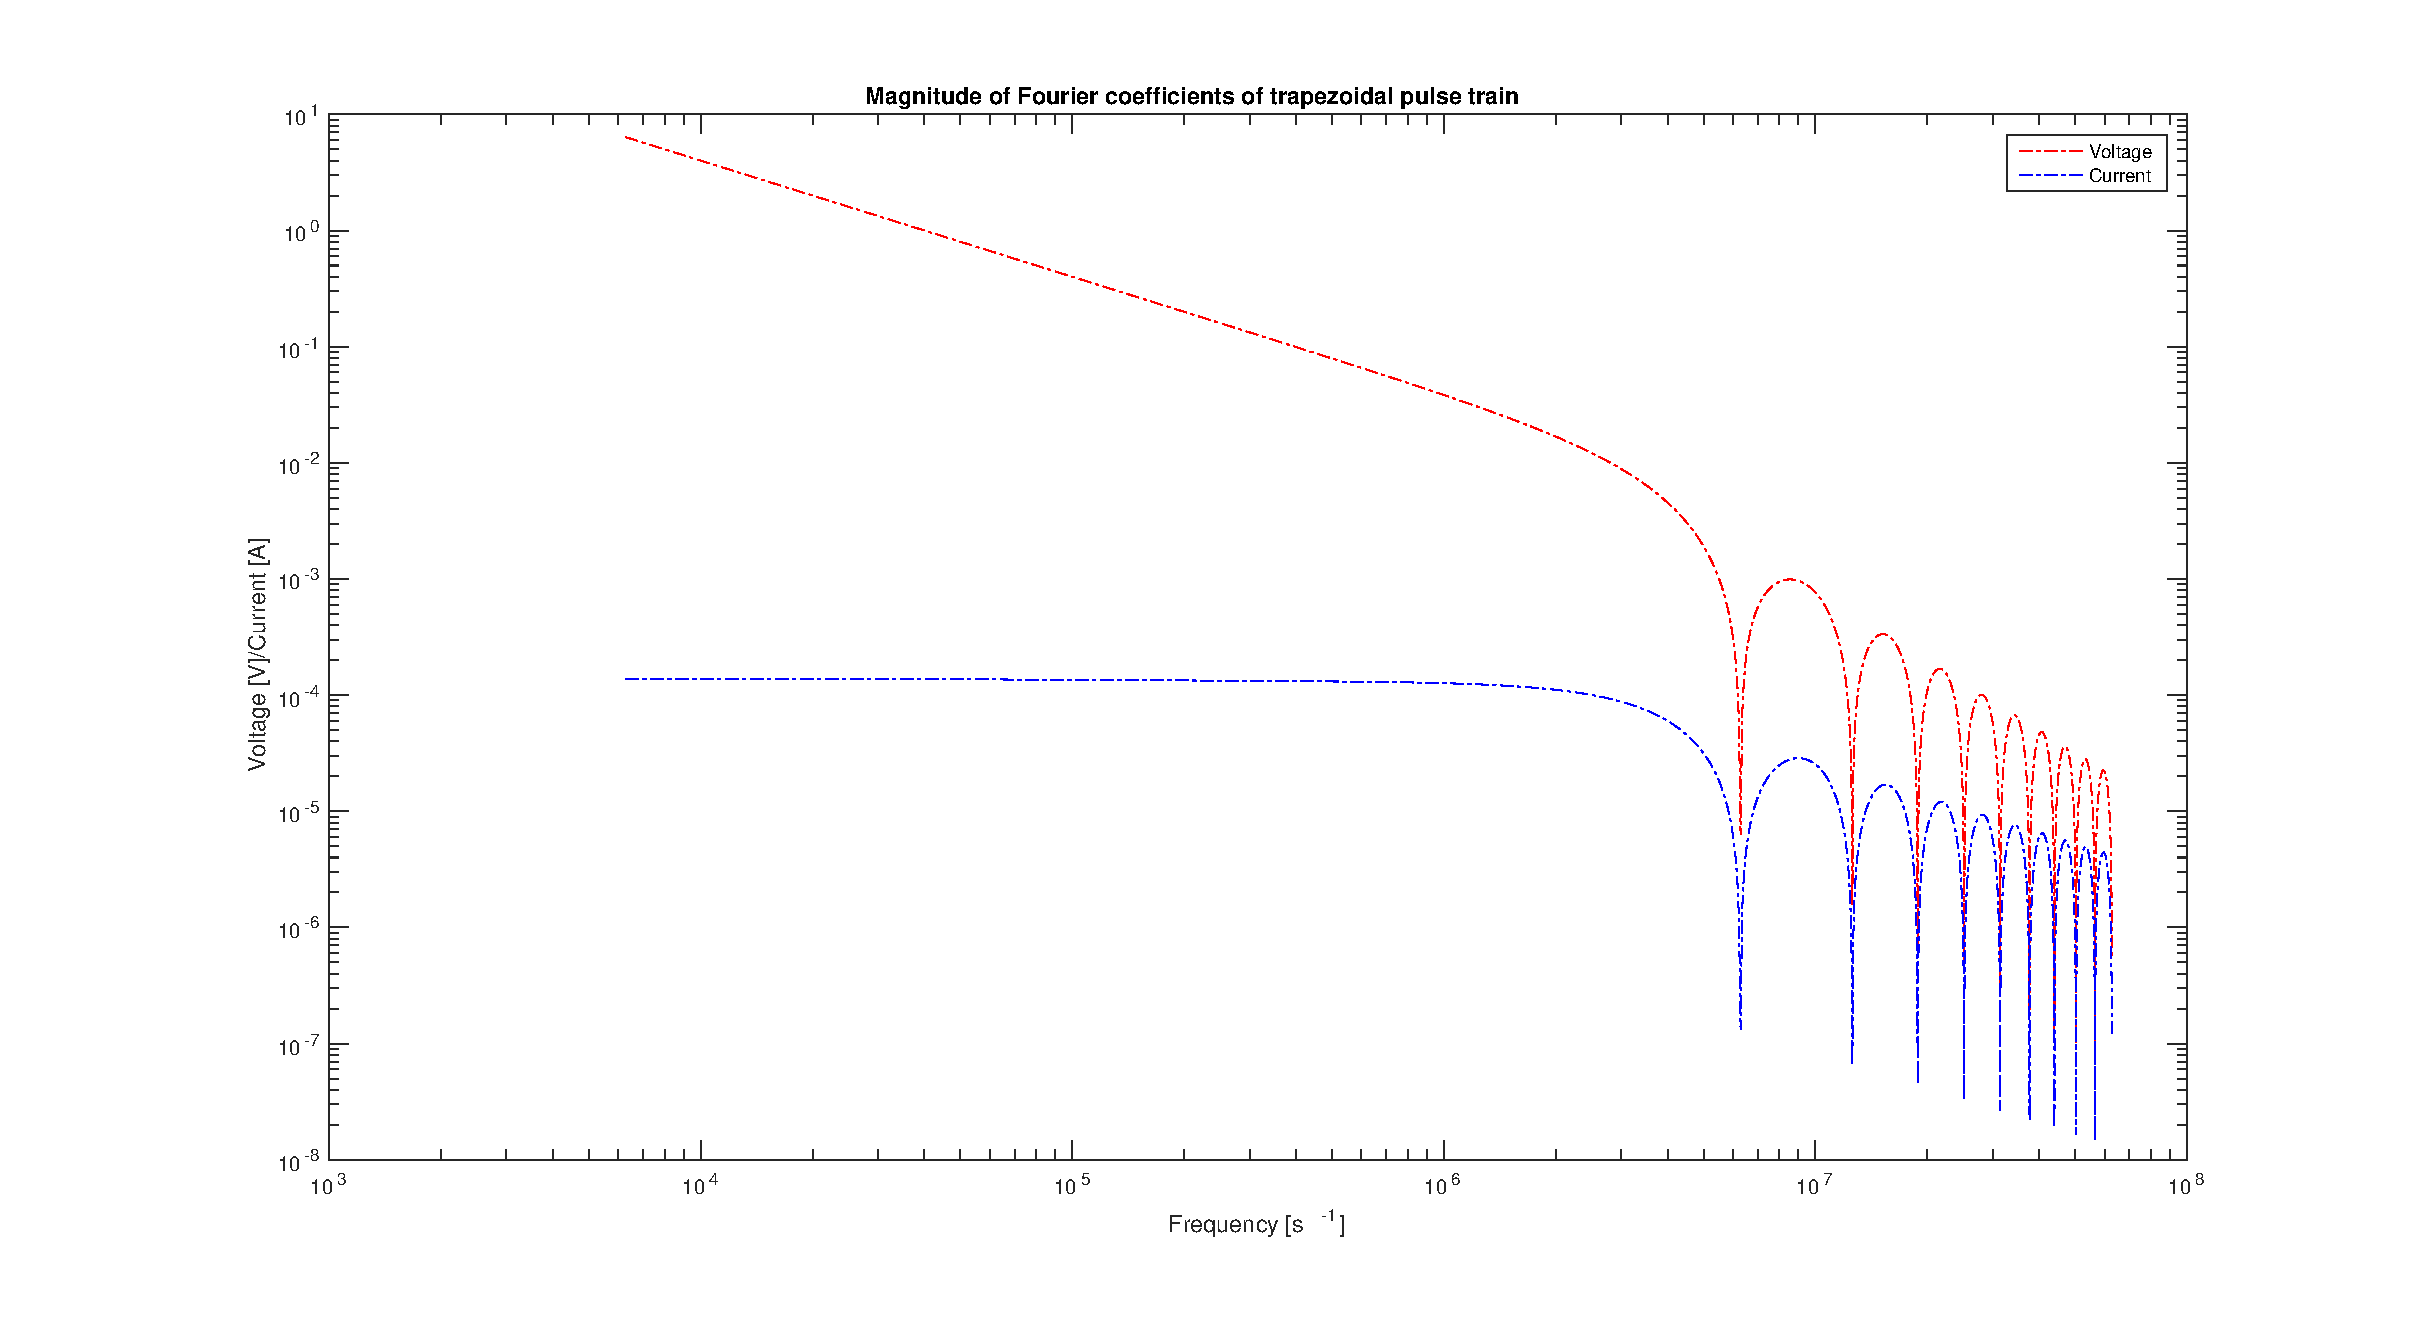
\includegraphics[width=\textwidth]{figures/Method/signal_simulation/fourierla.eps}}
\caption{Fourier coefficients of voltage applied to and current flowing through the Debye sample.}
\label{fig.fourierla}
\end{figure}

The current transformer has a nominal voltage to current transfer ratio of $\frac{1V}{1A}$. 
Consequentially the current signal that was determined before is now applied in the shape of a voltage to the input of the integrator (amplification of 1000 and upper cutoff frequency at 100 kHz) and subsequentially filtered by the low-pass filter in front of the positive input of the operational amplifier. 


\begin{figure}[h!tb]
\centerline{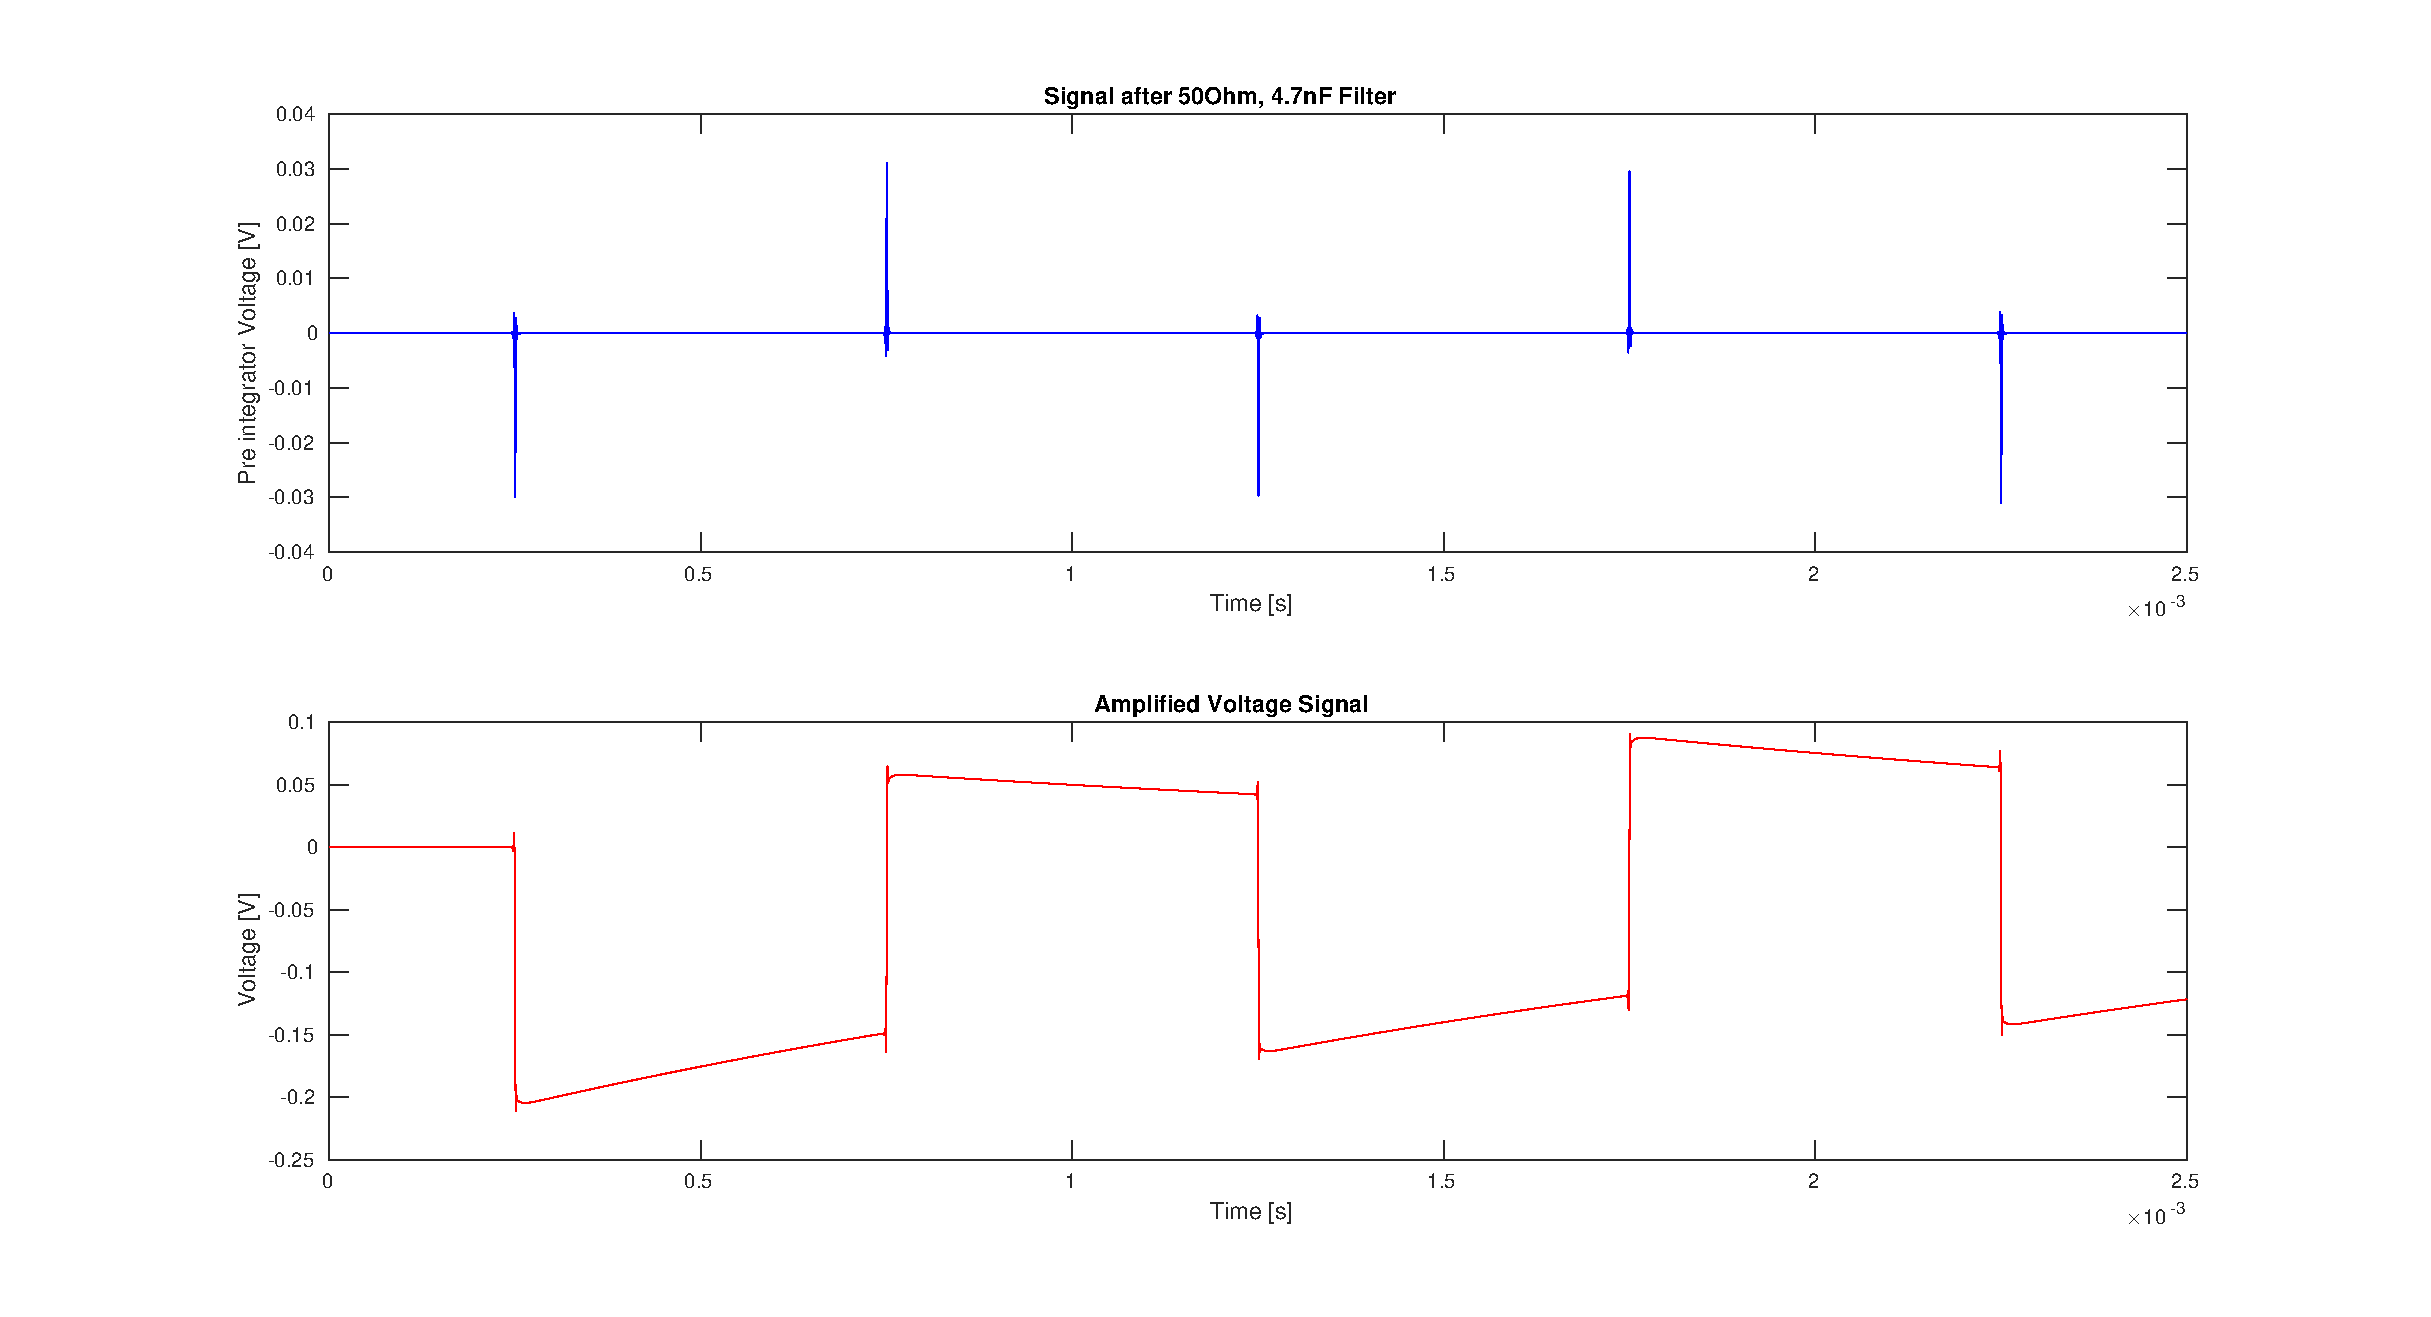
\includegraphics[width=\textwidth]{figures/Method/signal_simulation/integrated.eps}}
\caption{Signals before and after integrator}
\label{fig.integrator}
\end{figure}

In order to generate these signals, a simulation in Simulink was carried out using the components of the integrator circuit in \ref{fig.circuit}


Finally, a butterworth low-pass filter of $8^{th}$ order with an adjustable cutoff frequency
was installed \footnotemark. Its transfer function was applied to the FFT of the integrated voltage signal and the resulting 
signal is depicted in \ref{fig.finalvolt}
\footnotetext{Data Sheet for Butterworth Filter: data$\_$sheets$\/$USBPGF$\-$S1$\_$Data$\_$Sheet}

\begin{figure}[h!tb]
\centerline{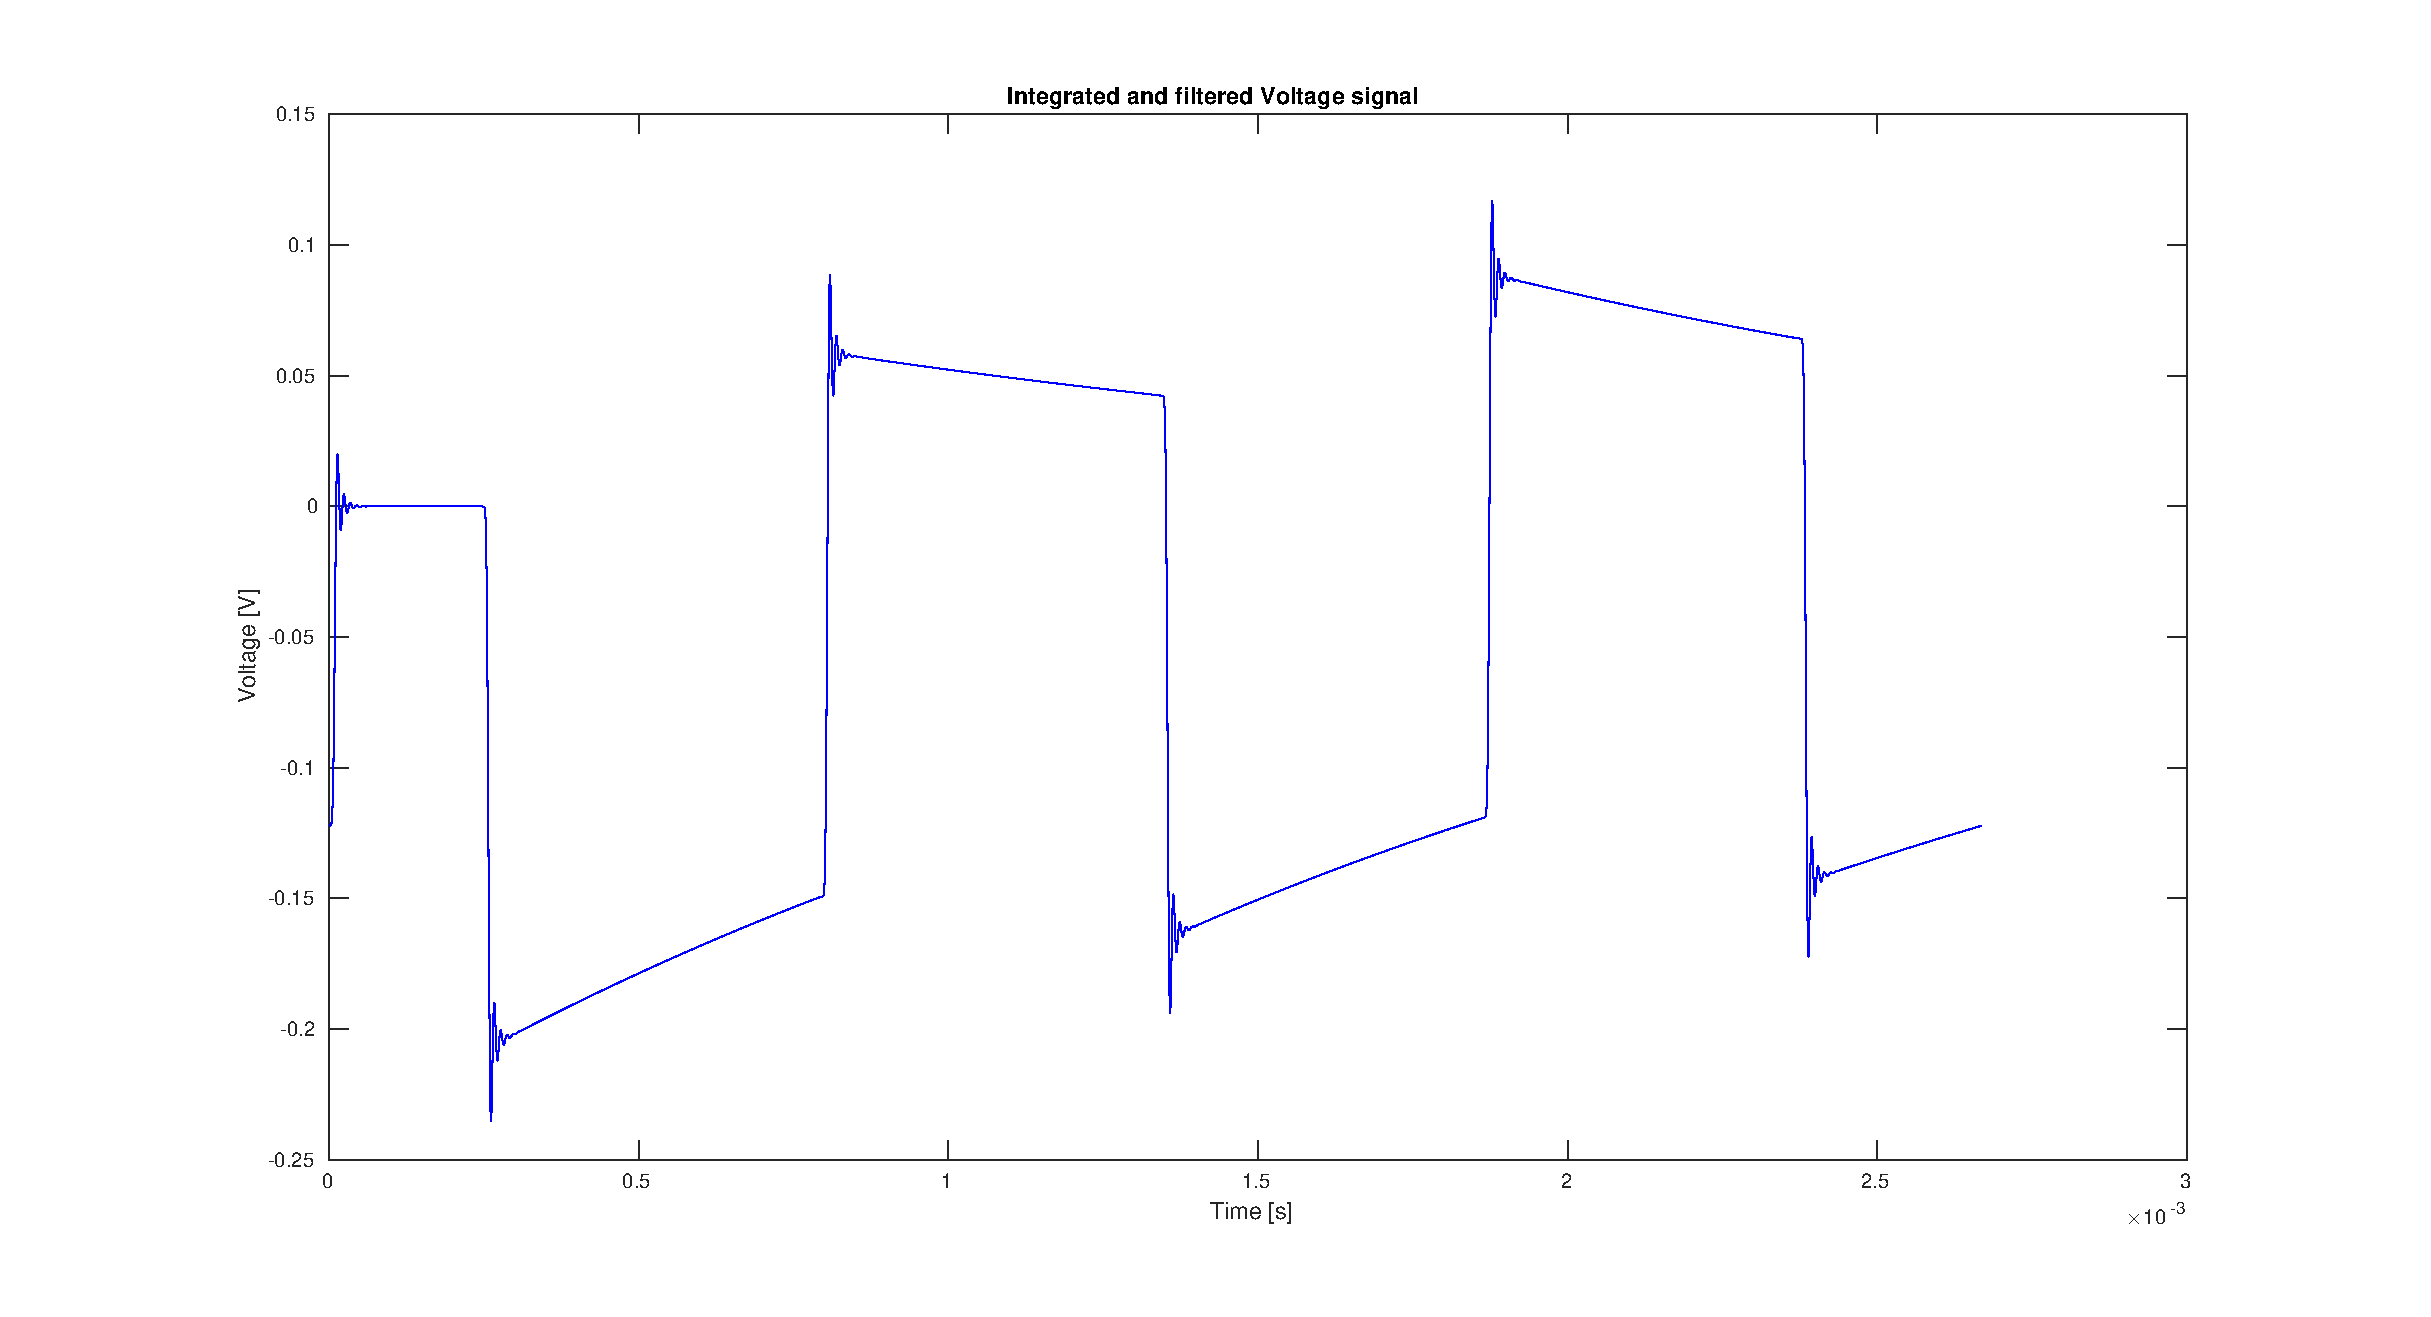
\includegraphics[width=\textwidth]{figures/Method/signal_simulation/finalvolt.eps}}
\caption{Final voltage signal to be measured by ADC}
\label{fig.finalvolt}
\end{figure}


\subsection{Design of a holder for the Debye Equivalent Circuit}
For a lossy medium the Debye Network consists at least of a vacuum capacitance $C_0$ and the term for the lossy charging of the additional capacitance. The DC resistance has a relatively high value and might therefore be left out, i.e. $R_{\infty}={\infty}$. It seems reasonable to design a holder for the network that can hold three strands with two components each. Moreover, it has to fit into the low-voltage and high-voltage test cell, which determined the dimensions of the holder.  
Figure \ref{fig.CADgraph} shows the created holder and a drawing is depicted in figure \ref{fig.CADdrawing}.

\begin{figure}[h!tb]
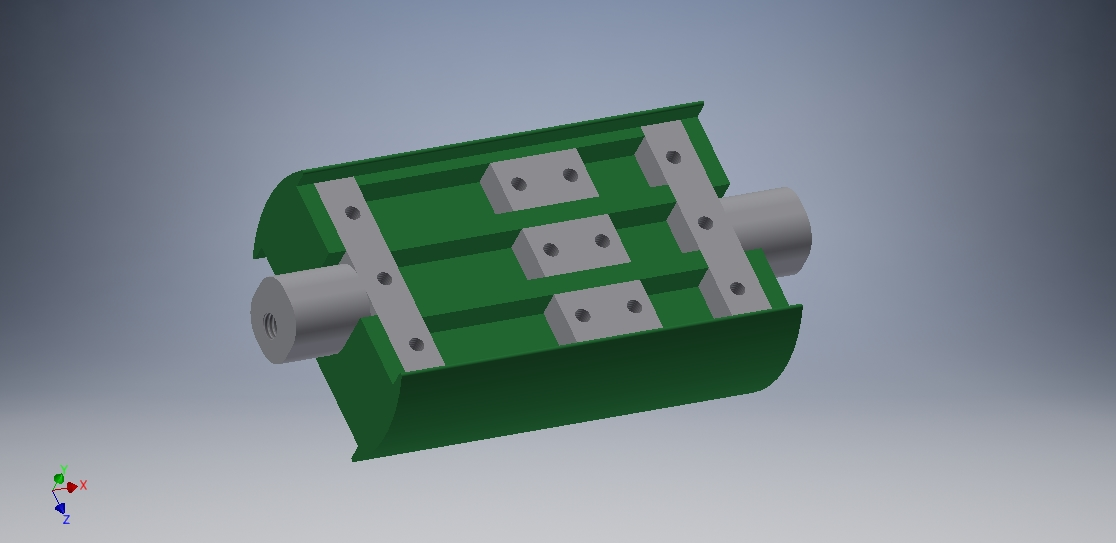
\includegraphics[width=\textwidth]{figures/Method/CAD_MODEL/Gesamtanordnung.jpg}
\caption{CAD representation for the holder of the Debye network. Created with Autodesk Inventor}
\label{fig.CADgraph}
\end{figure}




    

\subsection{Measuring of $\varepsilon_{\textrm{eff}}$ and tan($\delta_{\textrm{eff}}$) for the Debye model (dielectric spectroscopy)}
\label{spectroscopy}
The aim was to create a current through the Debye sample that is similar in shape and amplitude to the one expected in the high-voltage setup. In order to have a comparable current for a voltage that is $\frac{1}{1000}$ of the high-voltage setup a capacitance $C_0$ for the Debye is selected 1000 times higher than the capacitance of the samples. As the sample has a capacitance of approx. 3.5 pF its equivalent $C_0$ in the Debye model is chosen to be 3.3 nF.
A number of curves for the theoretical loss tangent, as well as their marked maximum frequency can be found in \ref{fig.debye-modell}.

The dielectric spectroscopy was conducted in the low-voltage setup and figure \ref{fig.presentation} can be used as a reference.
Generally, sinusoidal voltage signals were used in order to determine the effective relative dielectric permittivity.
The impedance method \cite{Kramer} approach was used to infere the permittivity given the signals in the setup.
In order to find the impedance of the setup, one has to compare the input voltage amplitude to the output current amplitude.

The course of action is described in this following passage.
\newline
A sinusoidal voltage signal with a variable amplitude is applied to the Debye model. There are in total 3 different measurement setups,
in the first setup the current is measured with the DLPCA, in the second, the current transformer is inserted for the purpose of measuring 
the current and in the third setup, that is similar to the second one, an integrator is added after the transformer in order
to achieve that both the input and the output's spectral components in the FFT analysis have the same $1/f$ dependency.
The digital signal processing unit or analog to digital converter (ADC) samples the signals in a way that 
the first component of the FFT's frequency corresponds to the fundamental frequency
of the sinusoidal wave generated by the function generator. Each measurement point is the result of 9 phase averages regardless of the frequency used.



\begin{equation}
\varepsilon(\omega)=\frac{I^*(\omega)}{i \omega \varepsilon_0 U^*(\omega)} = \frac{1}{i \omega Z^*(\omega) C_0}\\
\end{equation}
The ratio of the first component of the voltage's FFT divided by the first component of the current's FFT indicates the magnitude
of $Z^*(\omega)$ and a phase shift that deviates from 90 degrees will result in a complex relative dielectric permittivity. Then the loss tangent (as described in the theory section) can be determined. There are as well other phase shifts introduced by the BW-filter and the Current Transformer. These phase shifts, however, will cancel out as the measurement is divided by the results of the reference measurement which has these parasitical phase shifts as well. 
\newline
$C_0$ in the formula above denotes the vacuum capacitance and the associated impedance can be found by using the procedure described above with the difference that
the dielectric component, i.e. $R_i$ and $C_i$ are removed from the sample and only $C_0$ is left behind.

\begin{figure}[h!tb]
 \centering

 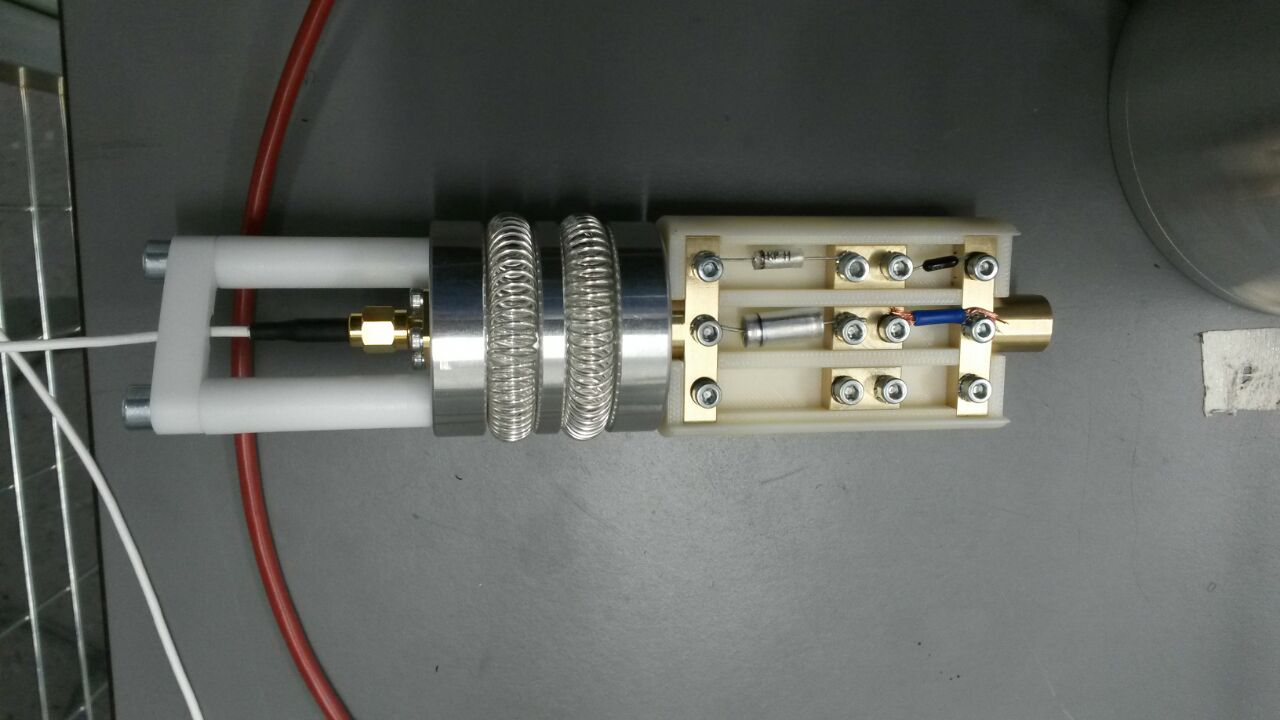
\includegraphics[width=0.5\textwidth]{figures/Method/Experimentaufbau/debyesample}
 \caption[Kurze Abbildungsbeschreibung]{Debye holder with components of Debye model inserted}

 
 
 \end{figure}

\begin{sidewaysfigure}[h!tb]
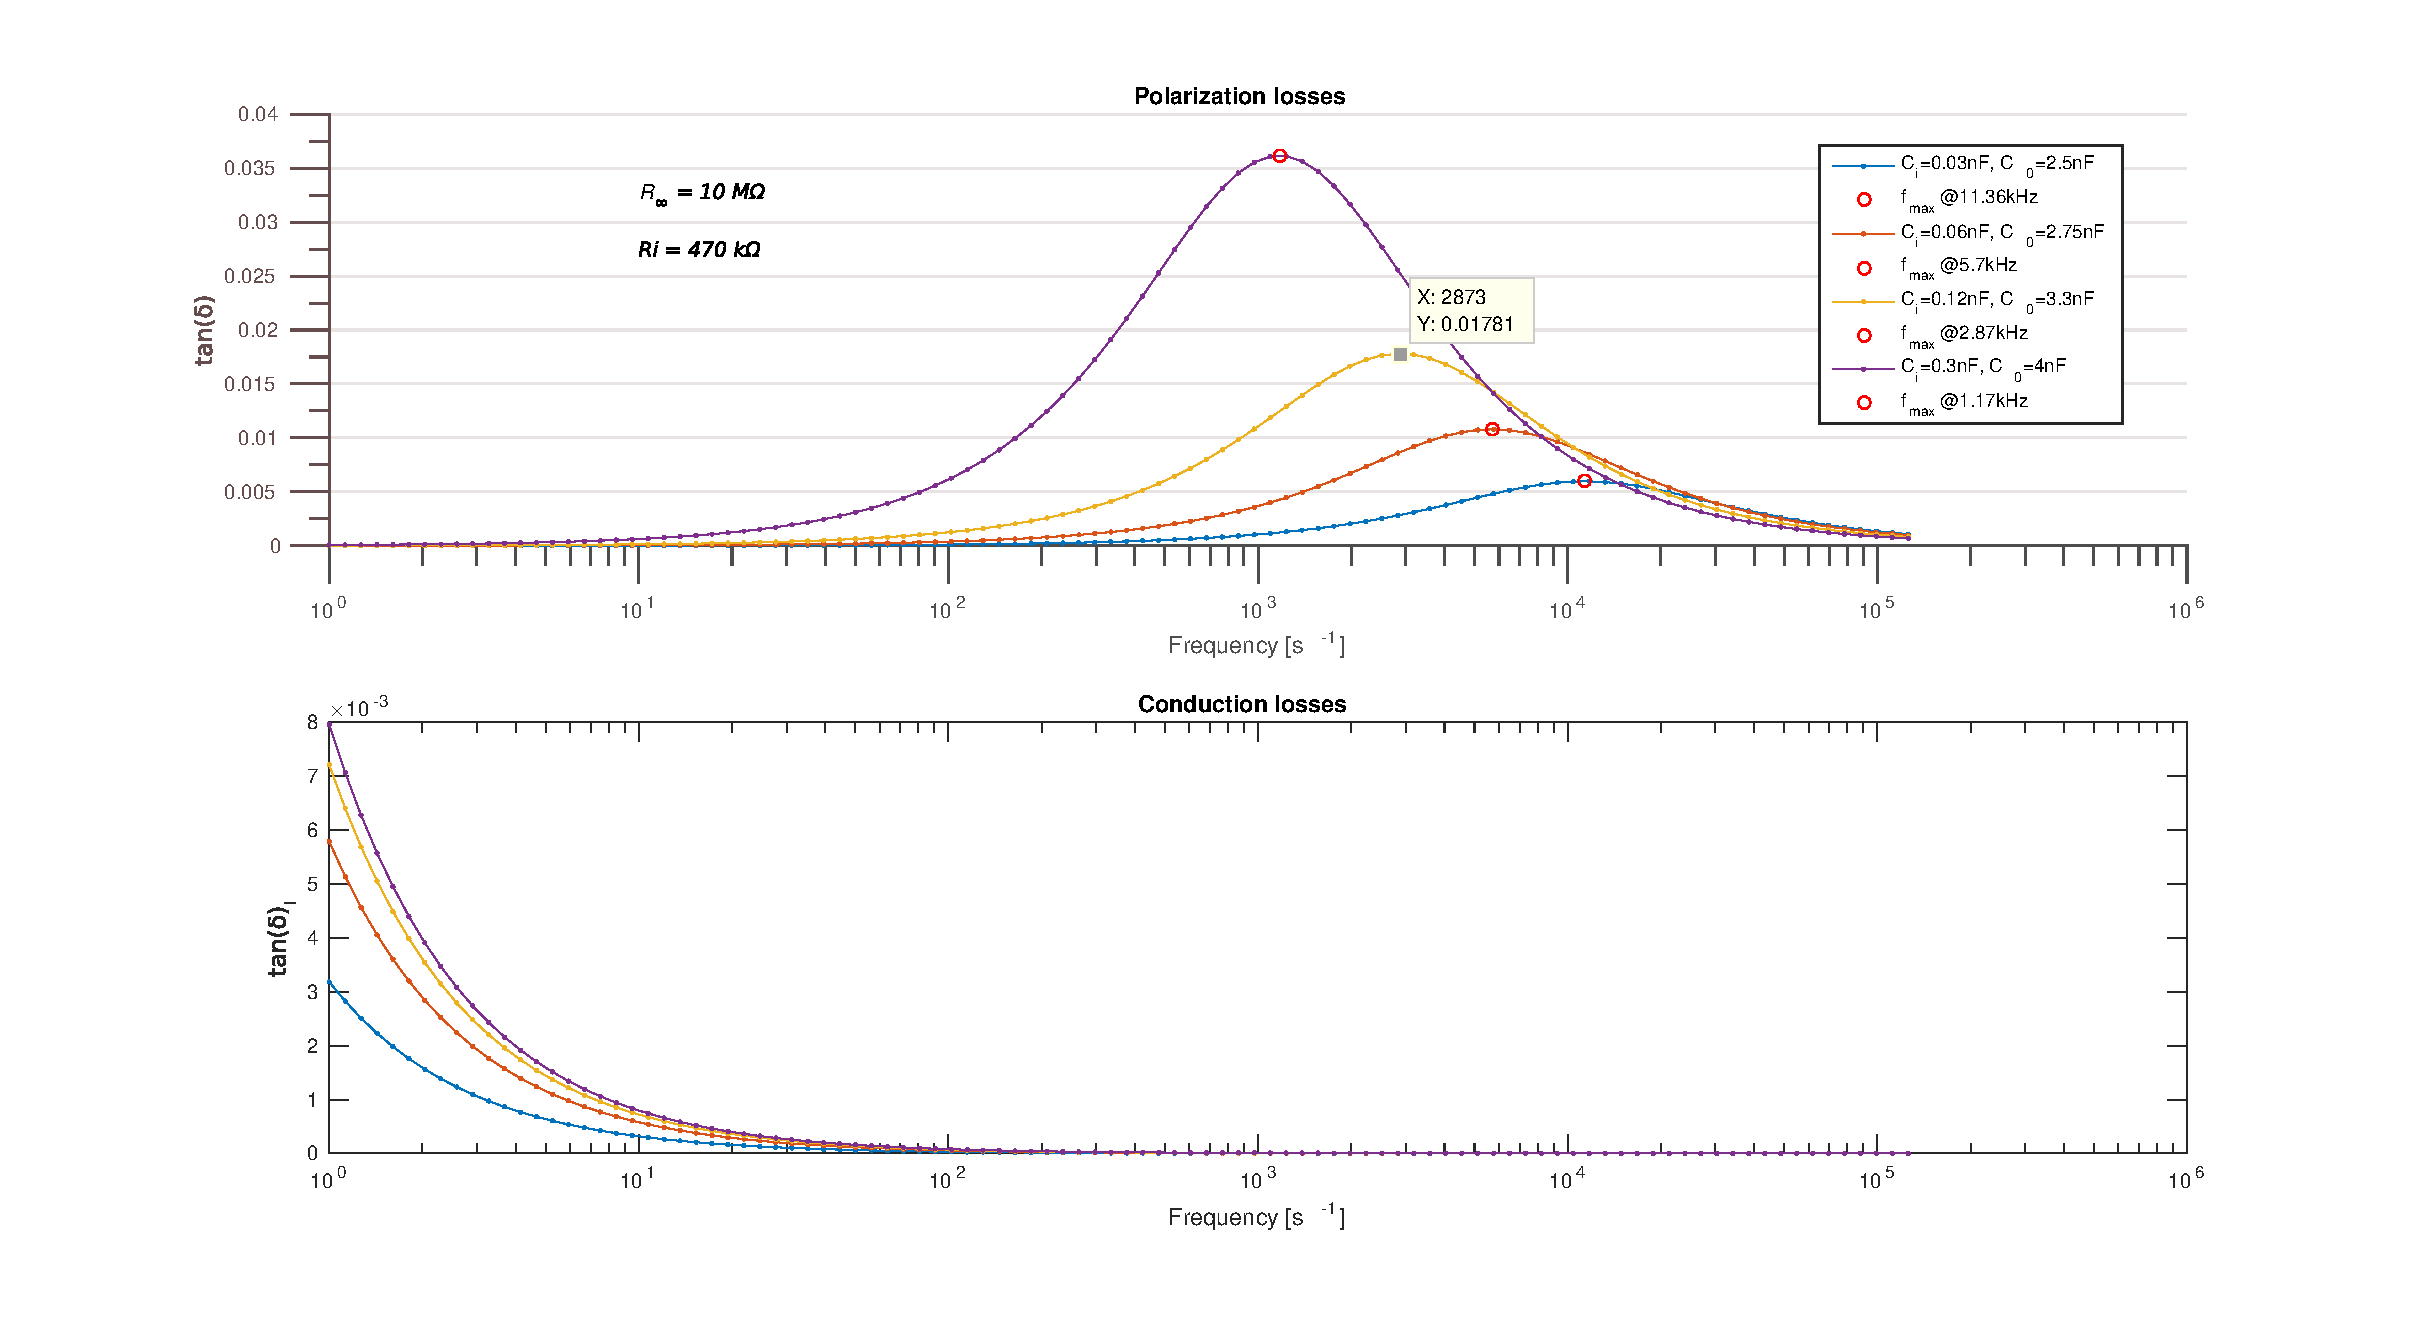
\includegraphics[width=0.99\textwidth]{figures/Method/Dielectric_loss/polarizationmultiple.eps}
    \caption{Polarization and conduction losses for different frequencies and different parameter values in the Debye model}
    \label{fig.debye-modell}
   \end{sidewaysfigure}

   
   \begin{sidewaysfigure}[h!tb]
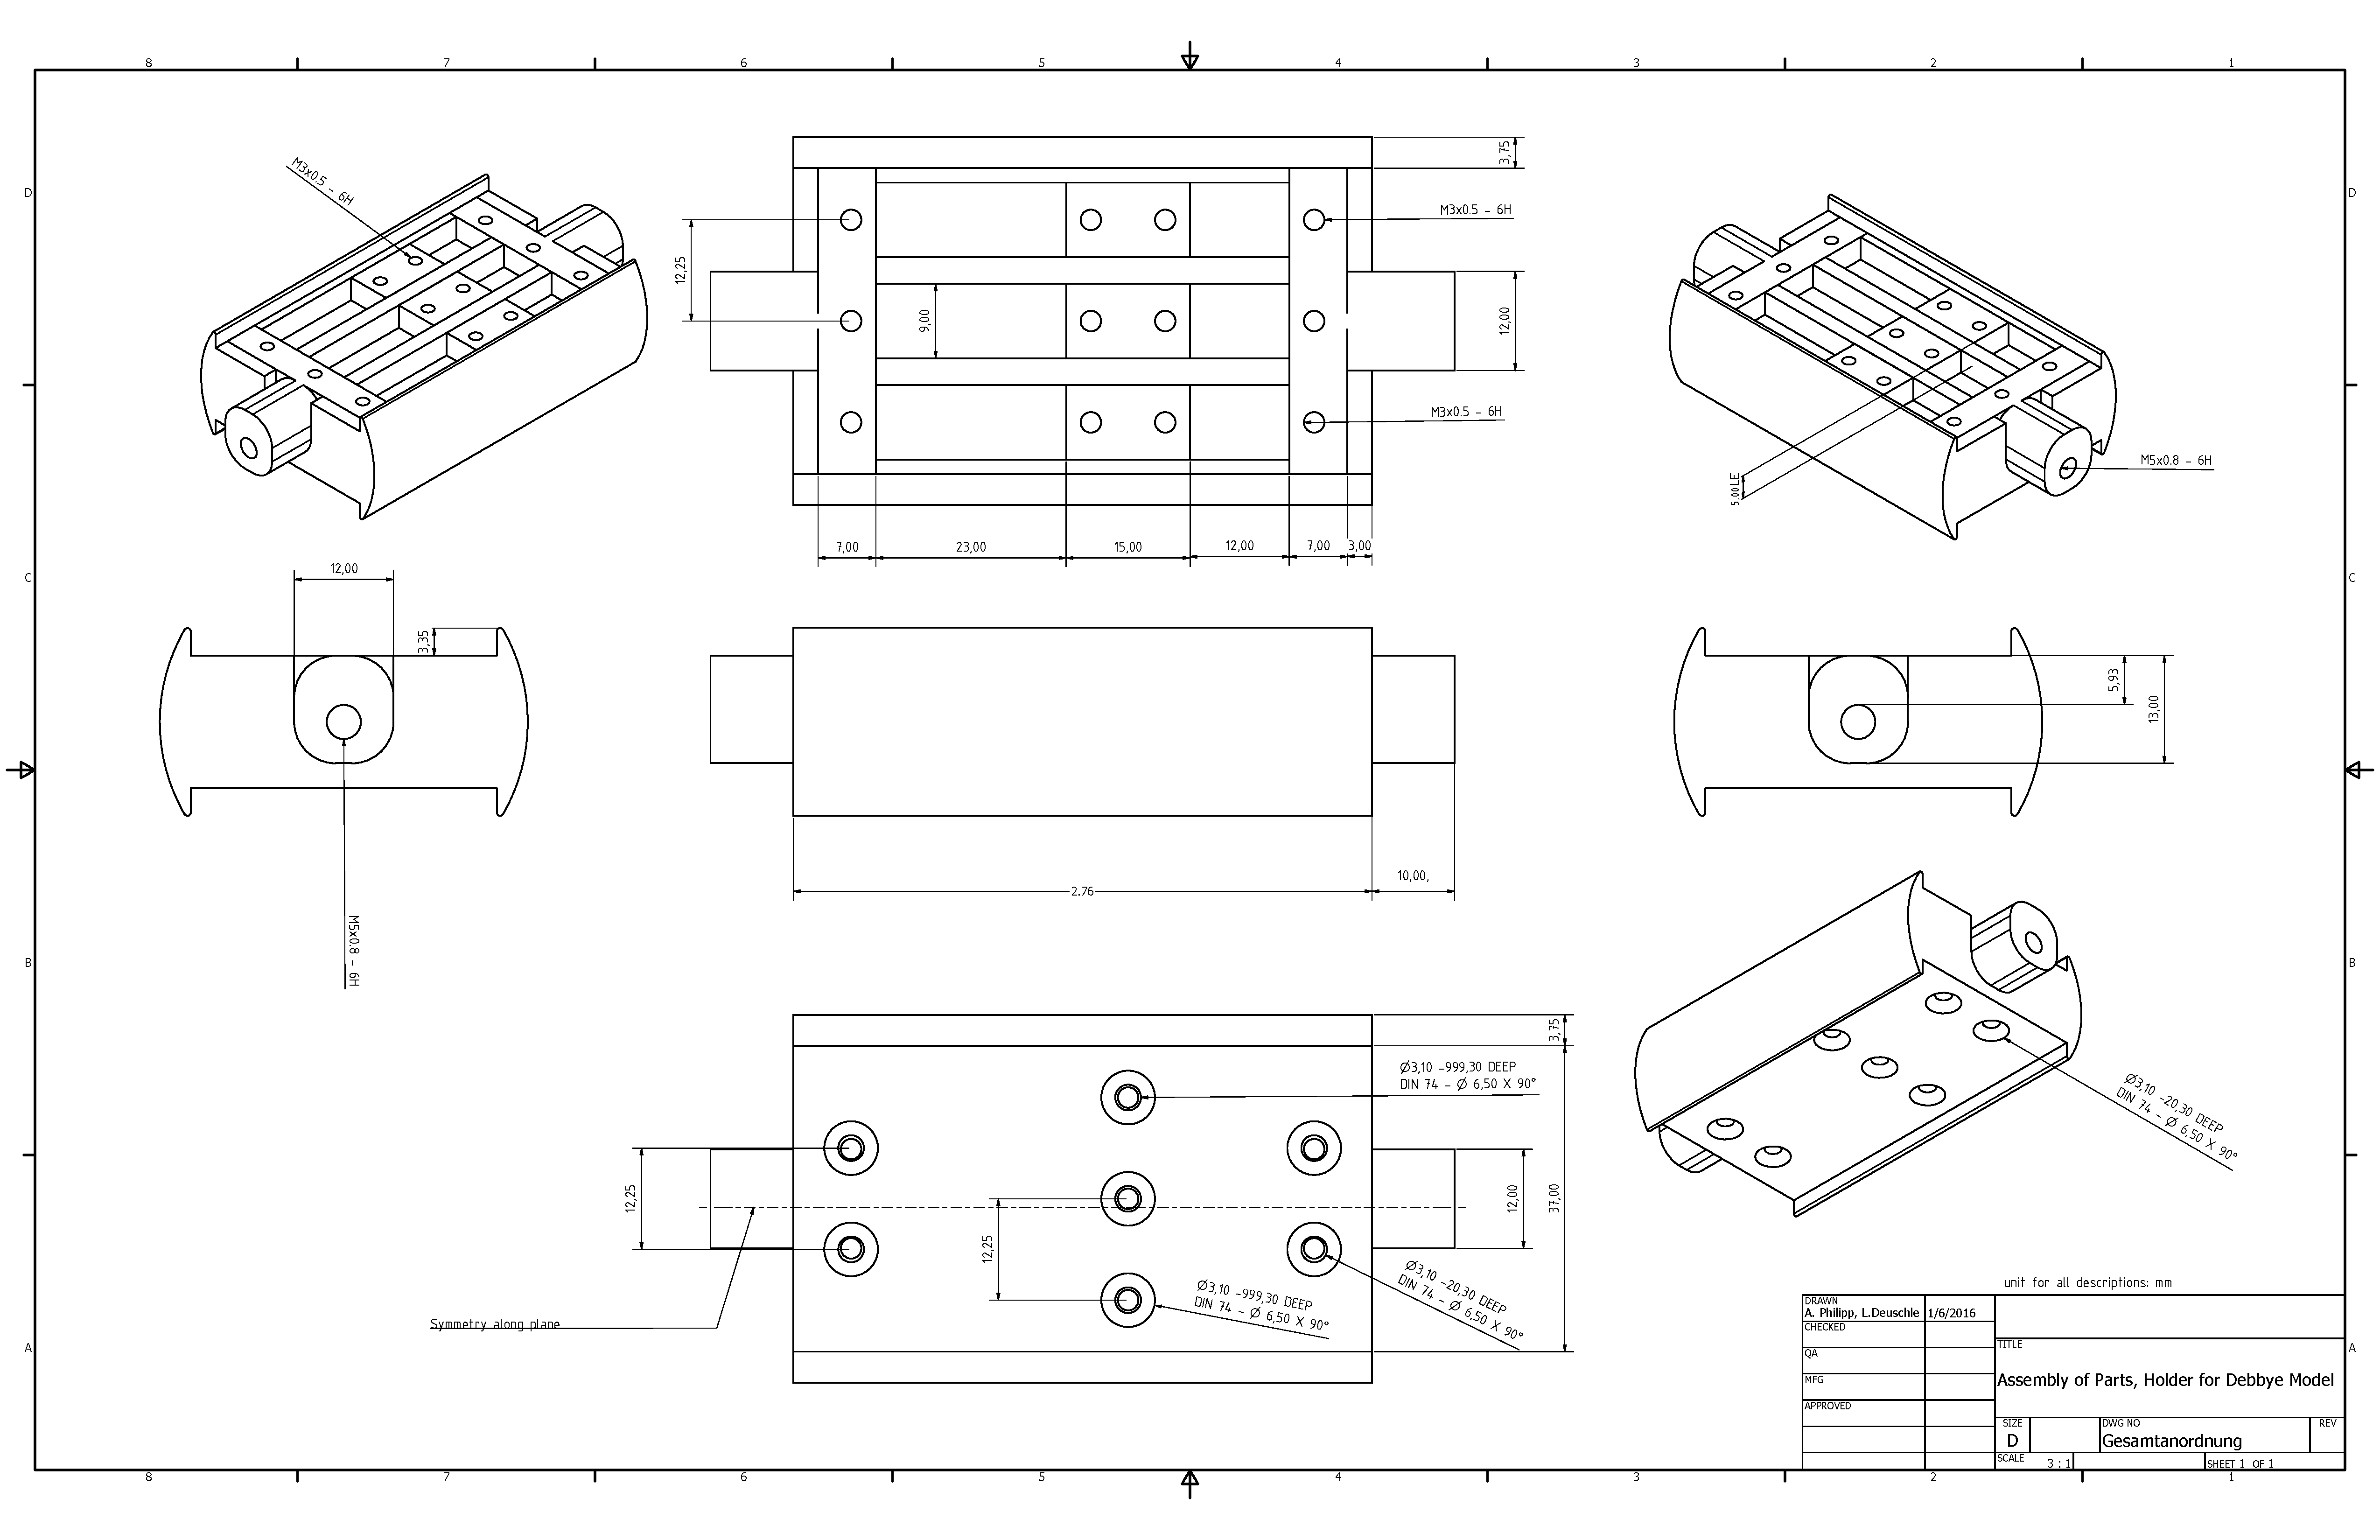
\includegraphics[width=0.99\textwidth]{figures/Gesamtanordnung.pdf}
    \caption{Drawing for the Debye sample holder}
    \label{fig.CADdrawing}
   \end{sidewaysfigure}

\subsection{Integrator}
\label{sec.integratormethod}
\subsubsection{Advantages of using an integrator}
As the used 16-bit ADC has a limited resolution it is advantageous to use an integrator in order to spread the Fourier components of the current signal over a larger timescale. This makes it possible to detect the different frequencies more accurately with the same ADC. 
A second reason to make use of an integrator is due to the fact that it adds an additional factor of $1/f$ to the Fourier spectrum of the output voltage signal. As the Fourier spectrum of the input signal is as well characterized by a $1/f$ decrease the integrator transforms the pulse signal back to a trapezoidal signal with a $1/f$-dependency in the Fourier spectrum. Since a $1/f$ dependency in the output signal is preferable to a constant Fourier spectrum due to better resolution for the first harmonics the integrator improves the measurement as well. 

\subsubsection{Design of the integrator}
\subsubsection{Functionality}
The integrator should have two functions. On the one hand side it should integrate the signal, on the other hand it should amplify the signal by a factor of approximately 1000. This is due to the fact that small currents ($\sim$mA) are to be measured. With a CT-sensitivity of $1V/A$ an amplification of 1000 is reasonable to use the full range of of the ADC of $\pm$ 10 V. \footnotemark These requirements can be achieved by a non-inverting integrator, which is shown in figure  \ref{fig.circuit}. 
\footnotetext{Data sheet of the used current transformer: Pearson Model 2877} 
\begin{figure}[H]
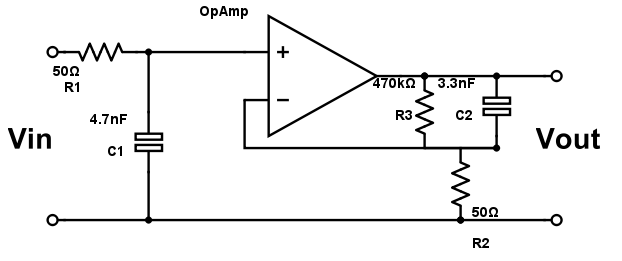
\includegraphics[width=0.99\textwidth]{figures/Method/integrator/circuit.png}
    \caption{Schematic non-inverting integrator circuit}
    \label{fig.circuit}
\end{figure}	

For the analysis of the transfer function of the integrator \ref{fig.circuit} is used as a reference.
At the input of the operational amplifier a low-pass filter is inserted to avoid integrating high-frequency noise.
The transfer function from the signal input to the positive input of the amplifier is given as

\begin{equation}
  G_1(s)=\frac{1}{1+sR_1C_1}
\end{equation}

The amplifier is set up in the non-inverting configuration, whose transfer function to the output is given by

\begin{equation}
 G_2(s)=\left[1+\frac{\left(\frac{1}{R_3}+sC_2\right)^{-1}}{R_2}\right]
\end{equation}

Combining the above results the following total transfer function is obtained:
\begin{equation}
	G_1(s)G_2(s)=TF_{int}(s)=\frac{1}{(1+s R_1 C_1)}\left[1+\frac{\left(\frac{1}{R_3}+sC_2\right)^{-1}}{R_2}\right]
\end{equation}
The transfer function of the integrator is illustrated by its bode plot (figure \ref{fig.Bodeplot}). 

\begin{figure}[H]
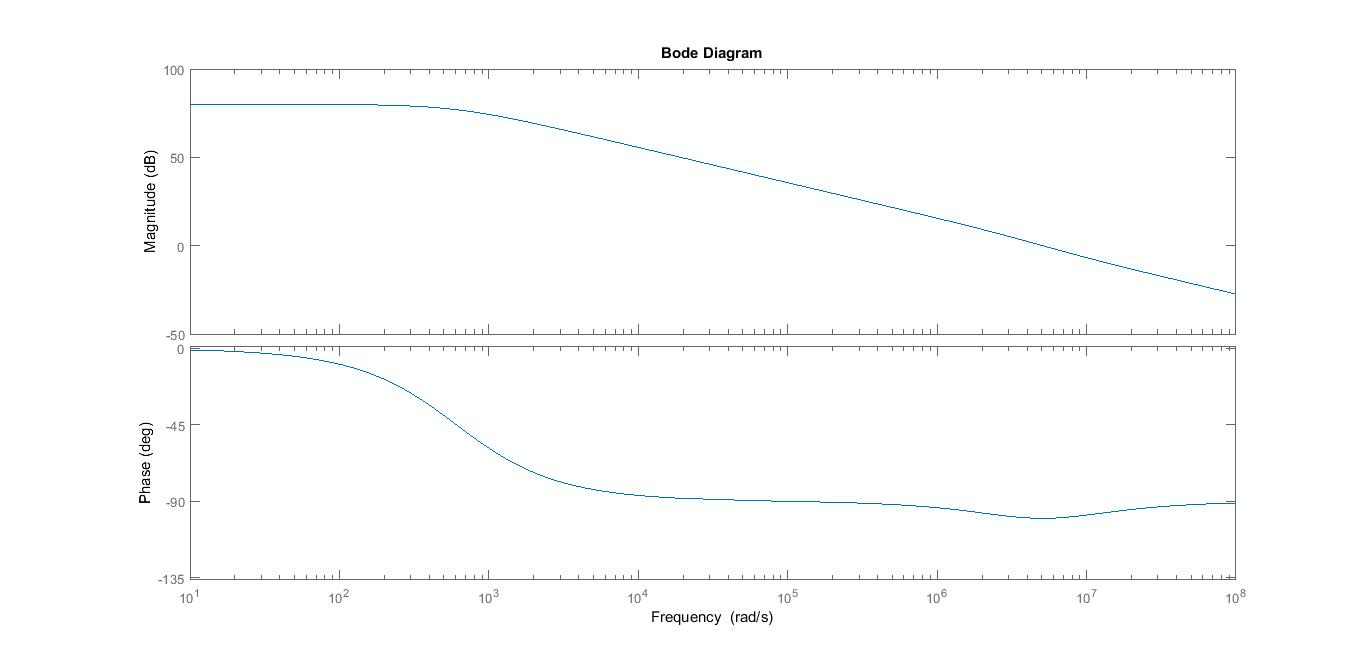
\includegraphics[width=\textwidth]{figures/Method/integrator/transferfunction_int.jpg}
\caption[Kurze Abbildungsbeschreibung]{Bode plot for the transfer function of the integrator}
\label{fig.Bodeplot}
\end{figure}

\subsubsection{Implementation}
The integrator together with its supply circuit were predominantely soldered on SMD footprints that were designed
with the PCB software EAGLE. The print can be found in \ref{fig.solder}.
The goal was to be able to operate the circuit with a unipolar voltage supply so an active charge pump in the 
shape of a 17-pin LTC3260 IC \footnote{/data$\_$sheets/LTC3260} was used to create the negative and positive supply voltage for the operational amplifier.\footnote{/data$\_$sheets/LT1028}
The circuit elements required for the charge pump were directly taken from the data sheet. The elements involved with the signal 
filtering and integration can be found in \ref{fig.circuit}
    
\begin{figure}[H]
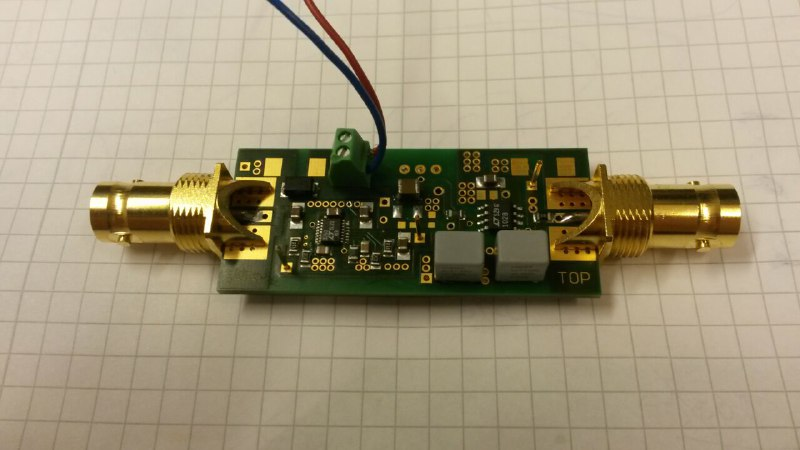
\includegraphics[width=\textwidth]{figures/Method/integrator/realintegrator.jpg}
\caption[Kurze Abbildungsbeschreibung]{Integrator circuit with BNC to SMD connectors}
\label{fig.realcircuit}
\end{figure}
\begin{sidewaysfigure}[h!tb]
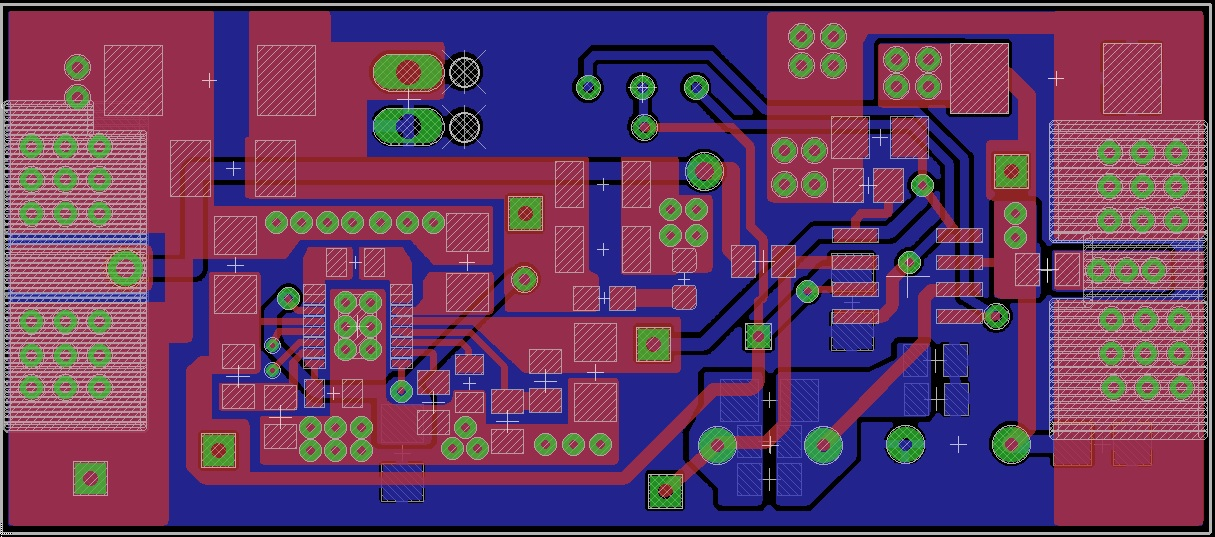
\includegraphics[width=0.99\textwidth]{figures/Method/integrator/PCB_Integrator.png}
    \caption{Printed Circuit Board Layout for the non-inverting ingrator with a DC voltage supply} 
    \label{fig.solder}
\end{sidewaysfigure}

    
    
    
\begin{sidewaysfigure}[h!tb]
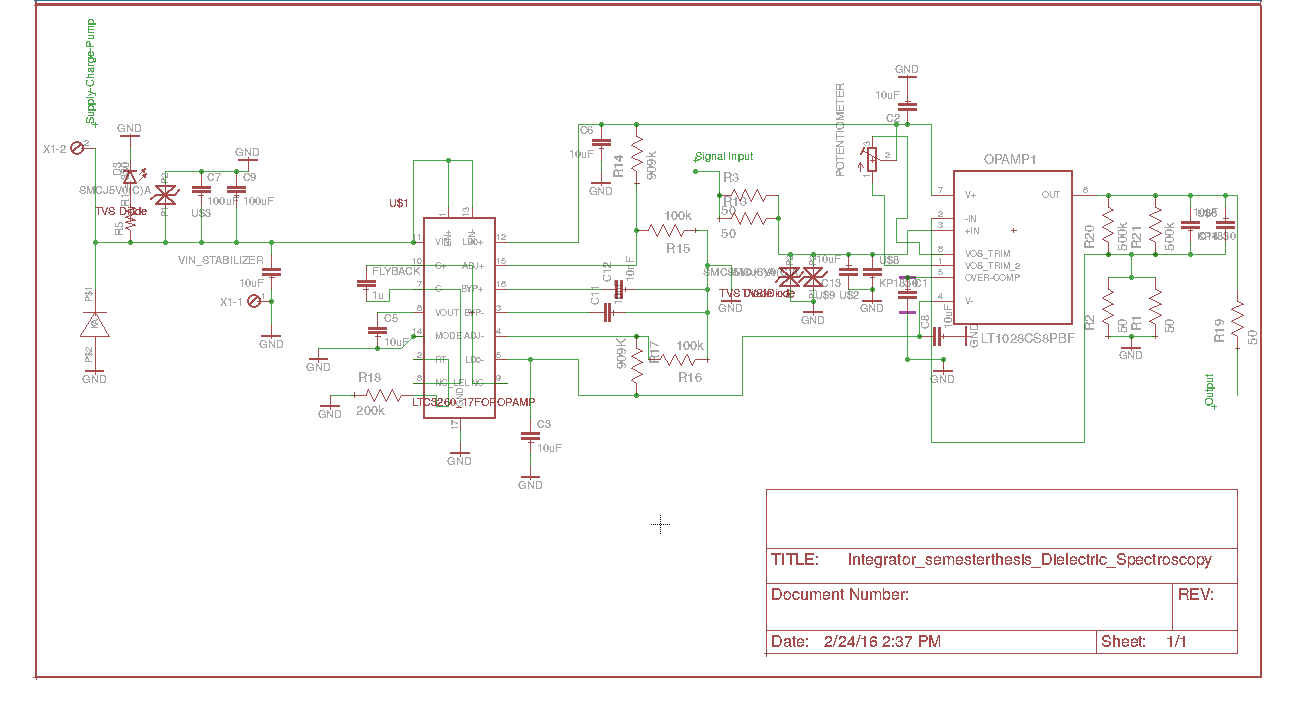
\includegraphics[width=0.99\textwidth]{figures/Method/integrator/schematic.jpg}
 \caption{Schematics for the Integrator circuit in EAGLE}
 \end{sidewaysfigure}


\subsection{Protective clamping capability of the current transformer}
\label{clamping}

In case of an object breakdown the sample loses its insulating properties and instead becomes conductive.
In this situation peak currents of several hundreds of amperes are expected to flow through the current transformer.
As a consequence, voltages of several hundred volts at its output will develop. In order to protect the sensitive electronics that
process and measure the signal after the transformer that was introduced in the section before a protective part has to be added.
A bidirectional TVS-Diodes (SMCJ7.0CA) \footnote{/data$\_$sheets/SMCJ7.0CA} connected to ground was used to clamp the voltage to a certain value regardless of what voltage the current transformer introduces.
To investigate the reliability of this setup, a measurement setup involving charged capacitor banks was used that could generate
pulses of currents with high amplitudes (up to 300 A). 
Primarily two performance parameters were to be investigated. First, are the TVS-diodes capable of clamping the voltage to their designated value even when
a variety of higher voltages were applied to them through the current transformer and secondly, how does the introduction of said TVS-Diodes affect the
signal transformation in case of normal operation. 
\newline
For this purpose a set of different current pulses was created and the performance of the current transformer was measured with the help of an
oscilloscope with and without the clamping setup. In order not to destroy the oscilloscope a -40dB resisistive attenuator was added in series in front of
the measuring port.

\begin{figure}[H]
\centerline{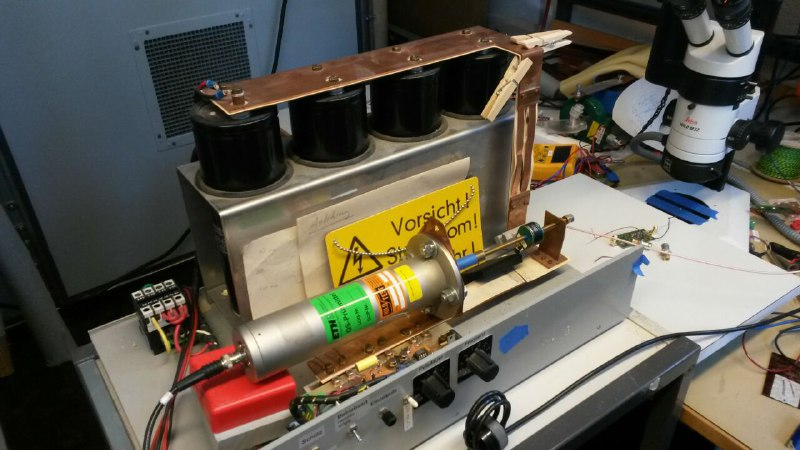
\includegraphics[width=0.8\textwidth]{figures/Method/Clamp/capacitorbank.jpg}}
    \caption{Capacitor bank that created the current pulses for the current transformer. Measurement of the voltage clamping}
    \label{fig.clamp}
\end{figure}



